%%%%%%%%%%%%%%%%%%%%%%%%%%%%%%%%%%%%%%%%%%%%%%%%%%%%%%%%%%%%%%%%%
%%% %
%%% % weiiszablon.tex
%%% % The Faculty of Electrical and Computer Engineering
%%% % Rzeszow University Of Technology diploma thesis Template
%%% % Szablon pracy dyplomowej Wydziału Elektrotechniki 
%%% % i Informatyki PRz
%%% % June, 2015
%%%%%%%%%%%%%%%%%%%%%%%%%%%%%%%%%%%%%%%%%%%%%%%%%%%%%%%%%%%%%%%%%

\documentclass[12pt,twoside,polish]{article}

\usepackage{weiiszablon}
\usepackage{polski}
\usepackage{graphicx}
\usepackage{cite}
\usepackage{caption}
\usepackage[table,xcdraw]{xcolor}
\graphicspath{ {./images/} }
\usepackage{xcolor}
\usepackage{listings}
\usepackage[utf8]{inputenc}
\usepackage{subcaption}
\usepackage[section]{placeins}
\usepackage{gensymb}
\usepackage{xurl}
\usepackage[autostyle]{csquotes}

\DeclareQuoteAlias{dutch}{polish}


\colorlet{punct}{red!60!black}
\definecolor{background}{HTML}{EEEEEE}
\definecolor{delim}{RGB}{20,105,176}
\colorlet{numb}{magenta!60!black}

\definecolor{deepblue}{rgb}{0,0,0.5}
\definecolor{deepred}{rgb}{0.6,0,0}
\definecolor{deepgreen}{rgb}{0,0.5,0}

\author{Rafał Ileczko}



\lstdefinelanguage{json}{
	numbers=left,
	numberstyle=\scriptsize,
	stepnumber=1,
	numbersep=8pt,
	showstringspaces=true,
	tabsize=2,
	breaklines=true,
	frame=lines,
	literate=
	*{0}{{{\color{numb}0}}}{1}
	{1}{{{\color{numb}1}}}{1}
	{2}{{{\color{numb}2}}}{1}
	{3}{{{\color{numb}3}}}{1}
	{4}{{{\color{numb}4}}}{1}
	{5}{{{\color{numb}5}}}{1}
	{6}{{{\color{numb}6}}}{1}
	{7}{{{\color{numb}7}}}{1}
	{8}{{{\color{numb}8}}}{1}
	{9}{{{\color{numb}9}}}{1}
	{:}{{{\color{punct}{:}}}}{1}
	{,}{{{\color{punct}{,}}}}{1}
	{\{}{{{\color{delim}{\{}}}}{1}
	{\}}{{{\color{delim}{\}}}}}{1}
	{[}{{{\color{delim}{[}}}}{1}
	{]}{{{\color{delim}{]}}}}{1},
}

\lstdefinelanguage{Python}{
	basicstyle=\fontsize{8}{10}\linespread{0.7},
	numbers=left,
	numberstyle=\scriptsize,
	stepnumber=1,
	numbersep=8pt,
	showstringspaces=true,
	tabsize=2,
	breaklines=true,
	frame=lines,
}


% np. EF-123456, EN-654321, ...
\studentID{EF-144087}

\title{Rozszerzona rzeczywistość we wspomaganiu obsługi urządzeń}
\titleEN{Augumented Reality in support of device operating}


%%% wybierz rodzaj pracy wpisując jeden z poniższych numerów: ...
% 1 = inżynierska	% BSc
% 2 = magisterska	% MSc
% 3 = doktorska		% PhD
%%% na miejsce zera w linijce poniżej
\newcommand{\rodzajPracyNo}{2}


%%% promotor
\supervisor{dr inż. Mariusz Oszust}
%% przykład: dr hab. inż. Józef Nowak, prof. PRz

%%% promotor ze stopniami naukowymi po angielsku
\supervisorEN{PhD Mariusz Oszust}

\abstract{Celem pracy było stworzenie systemu rozszerzonej rzeczywistości, pozwalającego na komunikację z dowolnym połączonym z siecią urządzeniem w przypadku wykrycia go na obrazie z kamery. Wykonana aplikacja pozwala na komunikację w czasie rzeczywistym dzięki protokołowi MQTT.}
\abstractEN{The puropse of this thesis was to develop an augumented reality system allowing to communicate with any external device connected to the network when detected in the camera's view. Developed application allow to real time communication via MQTT protocol.}

\keywords{wizja komputerowa, rozszerzona rzeczywistość, internet rzeczy, opencv, ar}
\keywordsEN{computer vision, augumented reality, iot, opencv, ar}

\begin{document}

% strona tytułowa
\maketitle

\blankpage

% spis treści
\tableofcontents

\clearpage
\blankpage


\section*{Wykaz symboli, oznaczeń i skrótów}
\begin{enumerate}
	\item[] \textbf{AI} Artificial Intelligence
	\item[] \textbf{AR} Augumented Reality
	\item[] \textbf{DL} Deep Learning
	\item[] \textbf{FLANN} Fast Library for Approximate Nearest Neighbors
	\item[] \textbf{IoT} Internet of Things
	\item[] \textbf{JSON} JavaScript Object Notation
	\item[] \textbf{MQTT} Message Queue Telemetry Transport
	\item[] \textbf{ORB} Oriented FAST and Rotated BRIEF
	\item[] \textbf{SIFT} Scale Invariant Feature Transform
	\item[] \textbf{SURF}  Speeded-Up Robust Features
	\item[] \textbf{VR} Virtual Reality
\end{enumerate}

\addcontentsline{toc}{section}{Wykaz symboli, oznaczeń i skrótów}%



\clearpage


\section{Wstęp}

Panującym obecnie trendem jest automatyzacja - słowo to występuje wielokrotnie na każdej konferencji. Dotyczy każdego rodzaju przemysłu i rynku usług. Jej efekty już od dawna odczuwamy także w życiu codziennym. Niczym dziwnym jest widok osoby mówiącej do telefonu, aby ten podał drogę do miejsca docelowego, wyszukał wykwintną restaurację, czy nawet opowiedział dowcip. Przedsiębiorstwa całego świata inwestują w działy automatyzacji produkcji zakupując kolejne manipulatory, czy też rozwoju, próbujące wymyślić nowe sposoby na wyeliminowania człowieka z procesu. W chwili obecnej to właśnie homo sapiens najsłabszym ogniwem. Maszyny, czy też oprogramowanie jest w stanie szybciej działać, wykonywać obliczenia będąc przy tym nieporównywalnie dokładniejszym. Jednocześnie urządzenia nie biorą urlopów, ich wydajność nie spada, nie wymagają motywacji, a także - co najważniejsze  mogą pracować 24h na dobę. Coraz częściej pojawiają się gniazda produkcyjne oraz magazyny w pełni autonomiczne, wymagające jedynie konserwacji.

Taka sytuacja ma miejsce nie tylko na obszarach produkcyjnych. W niektórych zawodach specjalizowanych coraz częściej modele sztucznej inteligencji mają lepsze osiągi niż specjaliści z dużym doświadczeniem. Tak jest na przykład w przypadku diagnozy niektórych schorzeń na podstawie danych o pacjencie oraz statystykach chorób \cite{healthcare}. W Estonii uruchomiono pierwszy na świecie sąd, gdzie wyroki dotyczą drobnych przestępstw wydaje model uczenia maszynowego \cite{judges}. W chwili obecnej takie narzędzia służą jako doradcy dla ludzi. Natomiast poprzez rozwój działu sztucznej inteligencji na świecie, będą pełniły coraz większą rolę. Można więc przewidywać, że w przeciągu kilku lat AI wyprze także specjalistów.

Jeśli obecne trendy się nie zmienią, w nowoczesnych procesach produkcyjnych będzie popyt na dwa typy pracowników: inżynierów tworzących nowe rozwiązania, oraz konserwatorów obecnych. Tutaj pole do automatyzacji jest mniejsze. Nie stworzyliśmy jeszcze sztucznej inteligencji tworzącej koncepcje nowych maszyn w sposób pragmatyczny, to jest uwzględniającej dokładną specyfikację. Podobnie ciężko zastąpić konserwatorów, którzy do pracy potrzebują zarówno zwinnych rąk, szeregu narzędzi jak i pomysłowości w diagnozie usterek. Mają oni jednak pewne zasadnicze ograniczenia. Posiadają zaledwie dwie ręce, oraz parę oczu mogącej patrzeć się w jedną stronę. Projekt wykonany w ramach niniejszej pracy stara się w pewnym stopniu znieść te ograniczenia, aby przyszli pracownicy mając do wykonania pewną pracę mogli skupić się na swoim zadaniu znacznie redukując liczbę obiektów potencjalnie go rozpraszających i ograniczających.

Odpowiednim rozwiązaniem powyższych problemów wydaje się być Rozszerzona Rzeczywistość (ang. Augumented Reality - AR). Metodologia ta polega na nałożeniu na obraz rzeczywisty widziany przez użytkownika elementów wygenerowanych przez program. Często spotykane zastosowania AR to filtry w aplikacjach typu Messenger czy Instagram. Pozwalają one wykonywać zdjęcia czy filmy ze zmodyfikowanym obrazem. Odpowiednie algorytmy poszukują ludzkiej twarzy na kadrze, a następnie modyfikują, dodając na przykład wąsy, bądź pogrubiając twarz. Innym częstym zastosowaniem są gry AR, gdzie najpopularniejszym przykładem jest Pokemon GO. Aplikacja wykorzystuje lokalizację użytkownika; będąc w miejscu gdzie występują pokemony można uruchomić aplikację, a na ekranie gracz zobaczy model 3D stworka z którym można nawiązać interakcję - walczyć, bądź go złapać. Rozszerzona rzeczywistość znajduje zastosowanie również w innych dziedzinach - firma Ikea udostępniła aplikację, która pozwala wizualizować jak będzie prezentował się dany produkt w otoczeniu użytkownika. Na potrzeby AR technologii powstały również specjalnie okulary, które pokazują wygenerowany obraz bezpośrednio przed oczami użytkownika, zamiast na ekranie.

Okulary AR są narzędziem nadającym się idealnie do celów konserwacji. Poprzez nałożenie na widoczny, rzeczywisty, obraz dodatkowych elementów możliwe jest bez oderwania wzorku od obiektu zainteresowania wykonać wiele czynności. Przykładowo dzięki będącemu zawsze w polu widzenia wskazaniu miernika, można testować obwody o wiele szybciej. Dzięki kamerze przebieg procesów można nagrywać, bądź współpracować zdalnie z inną osobą, gdzie obie widzą ten sam obraz. Przykłady można mnożyć, a dodatkową zaletą jest fakt, że nikt nic w ten sposób nie traci - wciąż możliwe jest wykonywanie wszystkich czynności w sposób tradycyjny.

Autor za wkład własny uważa:
\begin{itemize}
	\item Stworzenie oprogramowania pozwalające na spełnienie wizji opisanej w powyższym akapicie. Docelowo ma ono wspomagać obsługę i konserwację urządzeń dzięki metodom rozszerzonej rzeczywistości. Zakłada się, że dostępne maszyny, które mają być obsługiwane posiadają moduły umożliwiające połączenie się z lokalną siecią LAN, oraz mogą za jej pomocą wysyłać swoje parametry protokołem MQTT
	\item Stworzenie na potrzeby prezentacji pracy prostego urządzenia imitującego prawdziwe, dużo bardziej skomplikowane. A którego celem jest przesyłanie prostych wartości w postaci ciągu znaków.
\end{itemize}


\clearpage


\section{Wprowadzenie teoretyczne}

\subsection {Wirtualna i Rozszerzona Rzeczywistość}
W roku 2019 fotorealistyczna grafika komputerowa nie robi już na nikim większego wrażenia. Dzięki technikom Motion Capture generowane komputerowo postacie poruszają się zupełnie naturalnie. Specjalne algorytmy są w stanie symulować setki tysięcy włosów w czasie rzeczywistym \cite{hairworks}. Pierwsze gry wykorzystujące RayTracing są już na rynku gier komputerowych \cite{raytracinggames}, a badania nad dedykowanym sprzętem już się rozpoczęły \cite{raytracinghardware}. Oznacza to, że obecna technologia zbliża się do granicy fotorealizmu, jaki jesteśmy w stanie osiągnąć. Naturalnym rozwiązaniem wydaje się więc wyjście ze środowiska płaskich ekranów na rzecz bardziej naturalnych doznań.

Pierwszym znaczącym krokiem w tym kierunku była publiczna zbiórka pieniędzy na serwisie Kickstarter w 2012 roku na projekt Oculus Rift. Twórcy zebrali w ten sposób prawie 2,5 miliona dolarów amerykańskich na rozwój. Efektem ubocznym tego wydarzenia była znaczna popularyzacja terminu Wirtualna Rzeczywistość (ang. Virtual Reality - VR) wśród ludzi na świecie. Obecnie, a więc 7 lat od czasu zbiórki, do dyspozycji graczy dostępne jest 8 zestawów gogli VR, a liczba ta jeszcze się powiększy \cite{steamvr}. Wirtualna rzeczywistość jest technologią pozwalającą na prezentowanie użytkownikowi sztucznej, generowanej rzeczywistości. Dzięki specjalnym goglom, kontrolerom oraz technologii ich śledzenia, interakcja z otoczeniem dokładnie imituje rzeczywistą. Oznacza to, że ruch głowy użytkownika wywołuje identyczny ruch kamery w symulacji. Takie rozwiązanie pozwala na dużo większą interakcję użytkownika z otoczeniem niż jak ma to miejsce w symulacjach komputerowych wyświetlanych na typowym ekranie. W roku 2018 zyski firm z tytułu samego sprzętu VR przekroczyły 3,6 miliarda dolarów amerykańskich, co jest trzydziestoprocentowym wzrostem względem roku poprzedniego \cite{vr2018}. Zyski ze sprzedaży sprzęty VR w samym 2018 roku, z podziałem na kwartały prezentuje rysunek \ref{vrincome}.

\begin{figure}
	\centering
	\includegraphics[width=\textwidth]{vr2018}
	\caption{Zyski ze sprzedaży sprzętu VR w 2018 roku \cite{vr2018img}}
	\label{vrincome}
\end{figure}

Innym podejściem do tematu modyfikacji rzeczywistości jest rzeczywistość rozszerzona (ang. Augumented Reality). Technologia ta kompromisem pomiędzy rzeczywistością faktyczną, a wirtualną. Leży na środku osi, którą nazwać można \enquote{spektrum rzeczywistości}. Przedstawia ono jaka część danego rozwiązania jest rzeczywista, a jaka wirtualna (rys. \ref{realityspectrum}).

\begin{figure}
	\centering
	\includegraphics[width=\textwidth]{reality-spectrum}
	\caption{Spektrum rzeczywistości \cite{realityspectrum}}
	\label{realityspectrum}
\end{figure}

Jak widać na rysunku, AR znajduje się pomiędzy światem prawdziwym, a generowanym komputerowo. Jego celem nie jest wygenerowanie zupełnie nowej rzeczywistości jak ma to miejsce w przypadku VR, a jedynie stworzenie "wartości dodanej" do otaczającego świata. Przyjętą definicję AR zaprezentował Ronald Azuma. Rozszerzona rzeczywistość powinna objawiać się na trzech płaszczyznach \cite{azuma}:
\begin{itemize}
	\item Łączy świat rzeczywisty z wirtualnym
	\item Interakcja występuje w czasie rzeczywistym
	\item Rejestruje świat w trzech wymiarach
\end{itemize}

W przeciwieństwie do wirtualnej rzeczywistości, rozszerzenie może objawiać się na wielu typach urządzeń. Najbardziej powszechnym jest smartfon, jednak responsywność zapewniają okulary. Pozwalają one potencjalnie na zupełnie bezobsługowe ulepszenie rzeczywistości. Jednak zasadniczą zaletą technologii AR jest wykorzystanie obrazu do tworzenia modyfikacji. Dziękuje wykorzystaniu kamery, oprogramowanie jest w stanie przetworzyć obraz, wydobyć z niego pewne informacje, a następnie wykorzystać do stworzenia rozszerzeń obrazu. Dobrym przykładem takiej funkcjonalności jest wspomniana we wstępnie aplikacja Ikei na smartfony. Pozwala ona, wykorzystując kamerę telefonu, wyznaczyć płaszczyznę podłogi pokoju, a następnie dzięki odpowiednim obliczeniom wyrenderować model 3D produktu we właściwiej dla pomieszczenia skali i orientacji oraz zapamiętać położenie względem pomieszczenia. Jest to przydatne przy projektowaniu wnętrza pokoju, a możliwość poruszania się w takiej przestrzeni dopełnia wrażenia.

AR ze względu na swoją specyfikę dobrze odnajduje się w przemyśle. Raport firmy PTC \enquote{State of Industrial Augmented Reality 2019} \cite{ptcreport} twierdzi, że przemysł adaptuje najwięcej projektów AR, dzięki czemu wydajność pracowników gwałtownie wzrasta. Firmy oszczędzają również na szkoleniach, dzięki interaktywności rozwiązań.

\begin{figure}
\centering
\includegraphics[width=\textwidth]{arbyindustry}
\caption{Procentowy udział rynku w adaptacji projektów AR}
\end{figure}

\subsection{Dostępne narzędzia dedykowane AR}
\subsubsection*{Apple ARKit}
Narzędzie to stworzone przez Apple pozwala tworzyć aplikacje AR na urządzenia iPhone oraz iPad. Z tego też powodu miejsce ich zastosowań jest bardzo ograniczone - nie ma możliwości zaimplementowania swojego narzędzia na żadne z dostępnych okularów AR.

\subsubsection*{Google ARCore}
Kolejna biblioteka stworzona przez giganta branży IT. Jej wykorzystanie jest możliwe w systemach Android oraz iOS i w silnikach Unity oraz Unreal. Z tego też powodu doskonale nadaje się do tworzenia aplikacji AR na urządzenia mobilne.

\subsubsection*{Vuforia}
Jest rozbudowanym rozszerzeniem do silnika Unity. Pozwala rozpoznawać i śledzić płaskie oraz proste obiekty 3D w czasie rzeczywistym. Określa ich pozycję oraz orientację w przestrzeni, pozwala w prosty sposób nakładać na obraz obiekty 3D.

\subsubsection*{Wikitude}
Jest kompletnym narzędziem do tworzenia rozwiązań AR. Zawiera w sobie rozpoznawanie i śledzenie obiektów, geolokalizację, SDK pozwala tworzyć na urządzeniach mobilnych, oraz w Unity, Cordova, Titanium i Xamarin.

\vspace{5mm}

Istnieje również wiele innych mniej rozbudowanych rozwiązań. Autor, uznając jednak, że żadne ze wspomnianych nie spełnia jego oczekiwań, postanowił stworzyć własne.


\subsection{Zastosowanie AR w przemyśle}
Konserwacja jest procesem periodycznym, zajmującym mniej więcej tyle samo czasu, przy czym czas ten jest indywidualny dla każdej maszyny. Diagnostyka i naprawy występują rzadko, natomiast są czasochłonne, wymagają wykonania szeregu testów i pomiarów, aby diagnoza była możliwa. Wymagaj również szeregu dokumentów raportujących co zaszło, aby można było przeprowadzić stosowne analizy. Oba przypadki, choć skrajnie różne, mają cechę wspólną - poprzez ograniczenia ludzkie zajmują więcej czasu niż by mogły.

Najbardziej prymitywnym sposobem na usprawnienie pracy dzięki technologii jest zaopatrzenie pracownika w różnego rodzaju elektronarzędzia, tablet do sporządzania raportów i przeglądania instrukcji, czy krótkofalówkę do komunikacji. Są to rzeczy na pewno ulepszające proces, natomiast pewne na pewne rzeczy nie mają wpływu - człowiek wciąż musi samodzielnie wypełnić dokumenty, a podczas pracy może mieć szereg wskaźników, które musi śledzić na bieżąco, bądź podążać za procedurami, które nie zawsze da się dokładnie zapamiętać.

Dzięki technikom AR można część tych czynności ułatwić bądź zniwelować. Raport z operacji może zostać wygenerowany automatycznie dzięki nagraniu, bądź danym pobranym w jej trakcie. Testowanie obwodów może się odbywać bez odrywania od nich wzroku, dzięki pokazaniu pracownikowi bezpośrednio przed oczami wskazania miernika, bądź schemat. Nauka obsługi może się odbywać dzięki przedstawieniu zainteresowanemu każdego elementu urządzenia, z dodatkowymi informacji po wybraniu. Dzięki takim rozwiązaniom wydajność oraz dokładność wzrośnie, ponieważ nie człowiek będzie odpowiadał za część procesu, a dużo wydajniejszy program. Nie może zostać pominięty również czynnik ludzki, czyli zwykła pomyłka. Jej częstość zależy od wielu czynników, takich jak stan psychiczny człowieka, zmęczenie, czas pracy, czy zbliżające się terminy. W przypadku programów jest zgoła odwrotnie. Dobrze napisany będzie działał stabilnie, nie popełniając błędów. Dlatego też wspomaganie pracy programami komputerowymi wydaje się być szczególnie pożądane w newralgicznych momentach łańcucha produkcyjnego.

Jedną z firm, która wdrożyła rozwiązanie AR jest Avatar Partners. Celem stworzonego przez firmę rozwiązania było przyspieszenie nauki oraz konserwacji myśliwców armii Stanów Zjednoczonych. Stosując bibliotekę Vuforia stworzyli narzędzie, które było w stanie wizualizować położenie przewodów, systemu hydraulicznego i innym elementów. Według twórców czas potrzebny na wykonanie konserwacji został zmniejszony, naprawy przyspieszony oraz zredukowano liczbę popełnianych błędów. Dokładne liczby nie zostały jednak opublikowane. \cite{avatarpartnerscasestudy}


Firma Ingloba stworzyła dla Huawei Technologies narzędzie AR do wspomożenia instalacji i konserwacji paneli słonecznych Huawei. Stworzone narzędzie prezentowało kolejne kroki, które pracownik powinien poczynić, aby wykonać dane zadanie. Wykorzystanym urządzeniem jest tablet, więc istnieje możliwość sterowania programem poprzez ekran dotykowy. Poza wizualizacjami nakładanymi na rzeczywiste elementy, do dyspozycji pracownika są również tekstowe oraz filmowe instrukcje. Stworzono także listę kolejnych kroki procesu. Cała operacja jest rejestrowana i wysyłana na serwer w formie filmu. Według Huawei wdrożone rozwiązanie pozwoliło  operatorom lepiej zrozumieć wykonywane przez nich procesy, a same prace zaczęli wykonywać szybciej i dokładniej. \cite{huaweicasestudy}


\subsection {Sposoby zastosowań AR}
Rozszerzona rzeczywistość zakłada wykorzystanie kontekstu obrazu, który jest dostarczony do programu. Jednym z podejść do wykorzystania kontekstu jest stosowanie metod sztucznej inteligencji. Metody te służą do stworzenia modelu, który na podstawie dostarczonych danych jest w stanie nauczyć się wykonywać pewne zadanie. W przypadku problemu, który przedstawia poniższa praca, interesująca może być sekcja uczenia maszynowego, nazywana \emph{uczeniem nadzorowanym}. Metody te polegają na przekazaniu do modelu sztucznej inteligencji zbioru danych wraz z etykietami zawierającymi poprawną reakcję. Specjalne algorytmy wykonują swoje obliczenia na każdym obiekcie zbioru, a następnie sprawdzają, czy obliczenie jest poprawne. W zależności od odpowiedzi, modyfikują swoje parametry, aby wynik pokrywał się z dostarczonymi etykietami. Podstawowe algorytmy uczenia nadzorowanego mają jednak pewną zasadniczą wadę - są prymitywne i dla celów wizji komputerowej nie były najlepszych rozwiązaniem. Następcą prostych metod uczenia maszynowego jest uczenie głębokie (ang. Deep Learning - DL). Te metody są już szeroko wykorzystywane w projektach wizji komputerowej. Dzięki faktowi, że mogą wydobywać z obrazu unikalne cechy, zakres możliwości rośnie. Najpopularniejszym wykorzystaniem nauczonych modeli jest rozpoznawanie wielu klas obiektów na obrazie.

DL ma jednak kilka ważnych wad. Aby skutecznie nauczyć model wykonywać swoje zadanie, konieczny jest duży zestaw danych. Należy je odpowiednio przygotować, więc poza samymi zasobami, uczenie kosztuje również czas. Przyjmuje się, że dla każdej klasy obiektów, konieczne jest przygotowanie około 1000 zdjęć. Drugą wadą jest moc obliczeniowa, której zarówno do procesu uczenia, jak i późniejszego działania potrzeba dużo. Ostatnim minusem tego rozwiązania jest nieelastyczność. Modele uczenia głębokiego są typu \enquote{czarna skrzynka}, a więc zawierają parametry dla człowieka zupełnie niezrozumiałe i zakres działań, które można podjąć jest dosyć wąski - ogranicza się w zasadzie do douczenia modelu.

Innym podejściem do analizy kontekstowej obrazu jest \enquote{dopasowanie cech} (ang. feature matching). Polega ono na wydobyciu z obrazu specjalnych cech. Pobierając je z obrazu referencyjnego (obiektu, który chcemy wykryć) oraz obrazu z kamery (na którym jest poszukiwany obiekt), można je porównać i wyszukać czy i gdzie znajduje się obiekt referencyjny. Przewagą tej metody nad uczeniem głębokim jest fakt, że:
\begin{enumerate}[label=\alph*), leftmargin=1.25cm]
	\item wymaga mniej mocy obliczeniowej,
	\item nie wymaga uczenia,
	\item dzięki możliwości dostosowania parametrów wykrywania cech, elastyczność rozwiązania jest większa.
\end{enumerate}

Feature matching jest metodą wykorzystywaną nie tylko do rozpoznawania obiektów. Dzięki temu, że część wykrytych cech będzie się pokrywać na dwóch obrazach mających wspólny obszar, możliwe jest łączenie zdjęć w panoramy. Inne popularne zastosowanie do stabilizacja obrazu. Wiedząc, że kamera drga w osiach prostopadłych do osi głównej kamery, obraz końcowy można delikatnie przesuwać, dzięki czemu będzie on stabilny. Feature, jest unikalną cechą danego fragmentu obrazu. Mogą być to: krawędzie, narożniki, tekstury, koła i okręgi.

\begin{figure}[h]
	\centering
	\includegraphics{features}
	\caption{Potencjalne cechy}
	\label{features}
\end{figure}

Na rysunku \ref{features} wyodrębnione zostały trzy obszary: niebieski, czarny i czerwony. Pierwszy obszar nie wyróżnia się, nie jest więc unikalny. Podobnie sytuacja ma się w przypadku obszaru czarnego - tak samo wygląda cały obraz wzdłuż dolnej krawędzi zielonego prostokąta. Natomiast czerwony obszar jest unikalny, czyli nie ma drugiego takiego samego na rysunku. Wyszukiwanie unikalnych obszarów obrazu nazywa się detekcją cech (ang. Feature detection), a same cechy punktami charakterystycznymi (ang. keypoints). Kolejnym krokiem jest przetworzenie punktów, aby można było je porównać z tymi z innego rysunku. Taki proces nazywa się opisywaniem cech (ang. Feature description), a wynikiem tej operacji są deskryptory (ang. descriptors). Z punktu widzenia programu, zarówno punkty kluczowe jak i deskryptory są wektorami bądź tablicami asocjacyjnymi zawierającymi liczby. W dalszej części pracy opisane zostaną najpopularniejsze algorytmy obsługujące proces zarówno detekcji jak i deskrypcji.


\subsection{Algorytmy detekcji i deskrypcji}

\subsubsection[ORB]{ORB - Oriented FAST and Rotated BRIEF}

ORB jest metodą detekcji oraz deskrypcji punktów charakterystycznych wykorzystaną w poniższej pracy. Spaja ona detektor FAST oraz deskryptor BRIEF. Obie te techniki wyróżniają się niskimi wymaganiami mocy obliczeniowej. Autorzy tworząc to rozwiązanie podjęli się optymalizacji oraz zwiększenia odporności na zakłócenia.

ORB na początku wykorzystuje FAST do znalezienia punktów, następnie najmniej przydatne z nich są filtrowane za pomocą metody detekcji narożników Harrisa. Orientacja obszaru jest opisywana poprzez położenie wartości punktu nazwanego \enquote{intensywny centroid}. Zakłada się, że intensywnością jest przesunięcie narożnika od centroidu daje wektor jego orientacji. Sam centroid jest punktem geometrycznego środka danej figury. Deskrypcja odbywa się za pomocą algorytmu BRIEF. Ponieważ jednak nie radzi sobie on z rotacjami, wykorzystywane są te już obliczone dla punktów charakterystycznych. Każdy zestaw cech posiada $n$ binarnych testów w miejscu $(xi, yi)$, Tworzona jest dla nich macierz $S$ o rozmiarze $2 \times n$, zawierającą te współrzędne pikseli. Za pomocą orientacji cechy $\theta$ obliczona zostaje macierz rotacji, która po zastosowaniu obraca S, tworząc $ S_\theta $.

\begin{figure}
	\centering
		\includegraphics{orb_kp}
	\caption{Wykryte przez ORB cechy na przykładowym obrazie \cite{orbkp}}
\end{figure}

ORB dzieli cały obrót na obszary po $2\pi/30$ (12 stopni) i tworzy tabelę dla wzorców BRIEF. Dopóki orientacja punktu $\theta$ jest spójna pomiędzy obrazami, poprawny zestaw punktów $S_\theta$ zostanie użyty do wyliczenia deskryptora.

Każda cecha BRIEF posiada dużą wariancję i średnią bliską 0.5. Jednak gdy zostanie zorientowana wzdłuż wektora orientacji punktu, wartości te stają się bardziej rozproszone. Kolejną pożądana właściwością jest brak korelacji pomiędzy testami, aby nie wpływać na własne wyniki. W tym celu ORB przeprowadza przeszukiwanie zachłanne wśród wszystkich testów aby znaleźć te z dużą wariancją i średnią bliską 0.5, oraz brakiem korelacji. Metoda, ze względu na swoją szybkość i dokładność, została wykorzystana do stworzenia projektu realizowanego w ramach niniejszej pracy.

\subsubsection[SIFT i SURF]{SIFT - Scale Invariant Feature Transform oraz SURF - Speeded-Up Robust Features}
Inne popularne detektory i deskryptory to SIFT oraz SURF. Są to algorytmy opatentowane i płatne do komercyjnego zastosowania. SURF bazuje na SIFT i jest jest szybszą opcją.

Detektor narożników Harrisa jest w stanie wykryć narożniki niezależnie ich obrotu, jednak w przypadku zmiany skali sytuacja ma się inaczej. To co na małym obrazie jest narożnikiem, na dużym (dla badanych obszarów o jednakowej wielkości) jest tylko krzywą.

\begin{figure}[h]
	\centering
	\includegraphics{sift_scale_invariant}
	\caption{Porównanie narożników w różnej skali \cite{sift_scale_invariant_img}}
	\end{figure}

Rozwiązanie tego problemu opisał w 2004 roku D. Lowe z uniwerstyteu Kolumbii Brytyjskiej, w artykule \enquote{Distinctive Image Features from Scale-Invariant Keypoints} \cite{dlowe}, który poza wyznaczeniem punktów, oblicza również deskryptory. Na początku rozmiar obrazu jest podwajany za pomocą metod interpolacji. Następnie następuje iteracja rozmyć używając rozmycia Gaussa, z czego każdy kolejny obraz jest generowany ze zwiększonym odchyleniem standardowym. Następnie rozmiar obrazu jest zmniejszany dwukrotnie i występuje kolejna iteracja. Każda sekwencja iteracji pomiędzy pomniejszeniami obrazu nazywa się oktawą. Zjawisko to odbywa się do momentu w którym obraz jest zupełnie nieczytelny. Tworzona jest w ten sposób przestrzeń skali (ang. scale space). Jej celem jest symulowanie różnych skali obserwowanego obrazu. Każdy ze stworzonych rysunków jest normalizowany. Następnie zakłada się, przestrzeń skali ma trzy wymiary: koordynaty x, i y oraz odchylenie standardowe. Punkty kluczowe znajduje się za pomocą metody zwaną różnicą funkcji Gaussa. Dla każdego odpowiadającego sobie w ramach danej oktawy piksela wylicza się różnicę, a następnie wyznacza ekstrema. Wizualizacja tego działania przedstawiona jest na rysunku \ref{sift_gaussian}.

\begin{figure}[h]
	\centering
	\includegraphics[width=\textwidth]{sift_gaussian}
	\label{sift_gaussian}
	\caption{Schemat działania ekstrakcji cech \cite{sift_gaussian_img}}
\end{figure}

Wyznaczone punkty są następnie filtrowane. Konieczne jest wykluczenie krawędzi wśród wykrytych cech oraz punktów o niskim kontraście, aby zwiększyć stabilność. Dzieje się to za pomocą macierzy $H$, o rozmiarze $2 \times 2$, której wartości są proporcjonalna do krzywizny danego obszaru. Następnie do każdego punkty przypisywana jest orientacja. Tworzony jest histogram według orientacji gradientów wokół określonej cechy. Ma on 36 przedziałów, każdy odpowiada 10 stopniom. Każda wartość przedziału to wielkość gradientu i $1,5 * \theta$ (okno gaussowskie). Wybierane jest maksimum.

Kolejnym krokiem jest stworzenie deskryptora. Wybierane jest $16 \times 16$ pikseli wokół punktu. Obszar zostaje podzielony na 16 mniejszych o rozmiarze $4 \times 4$. Dla każdego małego obszaru tworzony jest histogram orientacji, łącznie 128 przedziałów. Wartości te finalnie przedstawione są jako wektor.

SURF jest bardziej wydajnym odpowiednikiem SIFT. Punkty kluczowe wyznaczane są za pomocą funkcji Hessa, a deskryptory zawierają informacji o ich położeniu i rozmieszczeniu.

\subsection{Dopasowanie cech}
Dopasowanie cech wykorzystuje się do rozpoznawania obiektu z obrazu referencyjnego na drugim obrazie. Ze względu na duża liczbę obliczeń w tym obszarze, wybranie optymalnego rozwiązania rzutuje w dużej mierze na szybkość całego systemu. 

\subsubsection{Brute-Force Matcher}
Najbardziej prymitywnym sposobem na dopasowanie jest \enquote{dopasowanie brutalne} (ang. Brute-Force). Realizuje się to poprzez porównanie deskryptora punktu do wszystkich deskryptorów z drugiego. Liczony jest dystans pomiędzy parami cech. Im jest on mniejszy, tym dopasowanie większe. Zwracana jest para o najmniejszym dystansie. W zależności od sposobu obliczania odległości, istnieją różne wersje algorytmu. Najpopularniejsze to \cite[s.573]{learnopencv}:

\begin{enumerate}[label=\alph*), leftmargin=1.25cm]
\item NORM\_L2, który wylicza odległość euklidesową pomiędzy cechami; stosowany dla algorytmów SIFT i SURF
\item HAMMING, wylicza odległość Hamminga (wykonanie XOR na ciągach binarnych i ich sumowanie); stosowany  dla binarnych rozwiązań jak ORB, BRIEF, BRISK.
\end{enumerate}

\subsubsection{FLANN based Matcher}
Inną metodą jest FLANN, będący akronimem od \enquote{Fast Library for Approximate Nearest Neighbors}. Zawiera w sobie zestaw algorytmów zoptymalizowanych pod proces poszukiwania najbliższych sąsiadów w dużych zbiorach danych oraz z wielowymiarowymi cechami. Metoda ta działa szybciej niż Brute-Force na dużych zbiorach i została wykorzystana w niniejszej pracy \cite[s.575]{learnopencv}.

\subsection[Model kamery otworkowej]{Model kamery otworkowej (Pinhole camera model)}
Podstawowy model kamery, zakładający, że wszystkie promienie światła zbiegają do jednego punktu - otworu kamery. Za jej pomocą wykonano pierwszą fotografię, przedstawiającą budynku rolnicze i niebo. Poniższy rysunek prezentuje zasadę działania takiej kamery.

\begin{figure}[h]
	\centering	
	\includegraphics[width=\textwidth]{pinhole_model_img}
	\label{pinhole_model}
	\caption{Geometryczny model kamery otworkowej \cite{cameralib}}
\end{figure}

Punkt zbiegu fal świetlnych jest w punkcie $O$. Główną osią jest $Z$. Płaszczyzna obrazu jest przesunięte od punktu $O$ o długość ogniskowej f. Punkt rzeczywisty P o współrzędnych $(X,Y,Z)$ rzutowany jest na płaszczyznę obrazu kamery na punkt $Pc=(u,v)$. Znając długość ogniskową oraz współrzędne punktu rzeczywistego, można wyznaczyć współrzędne punktu na obrazie.

$$ \frac{f}{Z} = \frac{u}{X} = \frac{v}{Y} $$
co po przekształceniach daje
$$ u = \frac{fX}{Z}$$
$$ v = \frac{fY}{Z} $$
Najczęściej tego typu obliczenia wykonuje się za pomocą macierzy, więc można powyższe równania zapisać jako
\begin{equation}
	\label{eq1}
	\begin{pmatrix} u \\ v \\ w \end{pmatrix}
	=
	\begin{pmatrix} f & 0 & 0 \\ 0 & f & 0 \\ 0 & 0 & 1 \end{pmatrix}
	\begin{pmatrix} X \\ Y \\ Z \end{pmatrix}
\end{equation}

Jeśli jednak oś Z nie przechodzi przez centrum obrazu z kamery, konieczne jest wykonanie translacji. Niech środek kadru reprezentuje $(c_u, c_y)$, wtedy
$$u=\frac{fX}{Z} + cx$$
$$v=\frac{fY}{Z} + cy$$
modyfikując równanie \ref{eq1} otrzymamy
$$
\begin{pmatrix} u \\ v \\ w \end{pmatrix}
=
\begin{pmatrix} f & 0 & c_x \\ 0 & f & cy \\ 0 & 0 & 1\end{pmatrix}
\begin{pmatrix} X \\ Y \\ Z \end{pmatrix}
$$

Ponieważ parametry rzeczywiste kamery podaje się w calach, konieczne jest przeskalowanie wartości do pikseli. Niech stosunek piksel/cal dla każdej z osi obrazu opisuje się wektorem $(m_x, m_y)$, wtedy 
$$
\begin{pmatrix} u \\ v \\ w \end{pmatrix}
=
\begin{pmatrix} m_x*f & 0 & m_u*c_x \\ 0 & m_y*f & m_y*c_y \end{pmatrix}
\begin{pmatrix} X \\ Y \\ Z \end{pmatrix}
=
\begin{pmatrix} \alpha _x & 0 & u0 \\ 0 & \alpha _y & v0 \\ 0 & 0 & 1\end{pmatrix}
*P = KP
$$
Macierz $\begin{pmatrix} \alpha _x & 0 & u0 \\ 0 & \alpha _y & v0 \\ 0 & 0 & 1\end{pmatrix}$ nazywa się macierzą parametrów wewnętrznych kamery i oznacza się literą K.

Jeśli punkt $O$ według danego układu współrzędnych nie leży w punkcie $(0,0,0)$, a oś $Z$ nie jest prostopadła do płaszczyzny obrazu, konieczne jest wykonanie translacji oraz rotacji. Macierz przesunięcia kamery do punktu $0$ to $T(Tx, Ty, Tz)$, a macierz rotacji obracająca kamerę do pozycji jak na rysunku \ref{pinhole_model} będzie nazwana macierzą rotacji R, o rozmiarze $3 \times 3$. Tworzona jest macierz
$$
E = (R|RT)
$$
nazwaną macierzą parametrów zewnętrznych, więc kompletnym równaniem transformacji jest
$$ K(R|RT) = (KR|KRT) = KR(I|T)$$
na punkt $P_c$ jest wyliczany przez
$$P_c = KR(U|T)P = CP$$
gdzie $C$ jest jest macierzą o rozmiarze $3 \times 4$ nazwaną macierzą kamery.

\subsection{Homografia}
Jeśli dwie kamery są zwrócone w kierunku jednego punktu, powiązanie pomiędzy nimi może być w prosty sposób obliczone. Rysunek \ref{homography-label} ilustruję sytuację, gdzie dla punktu $P\pi$, kamera 1 rzutuje go na obraz w punkcie $P^1_\pi$, kamera 2 analogicznie na $P^2_\pi$. Wiemy też, że punkt $P_\pi$ leży na płaszczyźnie $\pi$. Niech wektor normalny $N$ płaszczyzny będzie zdefiniowany przez $N = (a,b,c)$. Wtedy równanie płaszczyzny będzie równe:
$$ (N, 1) \cdot P = 0 $$
dla każdego punktu w świecie 3D.

\begin{figure}[h]
	\centering	
	\includegraphics[width=\textwidth]{homography_img}
	\label{homography-label}
	\caption{Przykład homografii \cite{cameralib}}
\end{figure}

Wiemy, że
$$P^1_\pi = \begin{pmatrix} u_1 \\ v_1 \\ w_1 \end{pmatrix} = C_1 \cdot P_\pi$$
Oznacza to, że punkt $P_\pi$ leży na promieniu $(u1,v1,w1,0)^T$, jednak parametr skali jest nieznany. Nazwiemy go $\tau$, otrzymując
$$ Ppi = \begin{pmatrix} u_1 \\ v_1 \\ w_1\\ \tau \end{pmatrix} = \begin{pmatrix}P^1_\pi \\ \tau \end{pmatrix}$$
Następnie, wiedząc, że $P_\pi$ spełnia równanie płaszczyzny otrzymujemy
$$ tau = -N \cdot P^1_\pi $$
,więc
$$ P_\pi = \begin{pmatrix} u1 \\ v1 \\ w1 \\ \tau \end{pmatrix} = \begin{pmatrix} I \\-N \end{pmatrix} P^1_\pi $$
$I$ jest macierzą $3 \times 3$, $N$ $1 \times 3$, więc otrzymana jest macierz $4 \times 3$.
Niech $C_2 = \begin{pmatrix} A_2 & a_2\end{pmatrix}$, gdzie $A_2$ to macierz $3\times 3$, a $a_2$ wektor $3 \times 1$. Wtedy,
$$ P^2_\pi = C_2 \cdot P_\pi = \begin{pmatrix} A_2 & a_2\end{pmatrix} \begin{pmatrix}I \\ -N \end{pmatrix} P^1_\pi $$
Macierz $C_2$ ma rozmiar $3 \times 4$, kolejna $4 \times 3$, więc wynikiem jest macierz $3 \times 3$, nazywaną macierzą homografii. Ostatecznie
$$P^2_\pi = (A_2-a_2 N)P^1_\pi = HP^1_\pi$$

Macierz homografii pokazuje relację pomiędzy obrazem z dwóch kamer. Używając jej, możliwa jest transformacja widoku, aby odpowiadał położeniu drugiej \cite[s.660]{learnopencv}.


\subsection{Zastosowane technologie}
\subsubsection{OpenCV}
Najważniejszą technologią zastosowaną w niniejszej pracy jest OpenCV. Jest to popularna otwarta biblioteka o otwartych źródłach służąca do przetwarzania obrazu, stworzona przez firmę Intel. Oficjalnie projekt rozpoczął się w 1999 roku. Obecnie zawiera w sobie  ponad 2500 algorytmów rozwiązujących zarówno typowe problemy wizji komputerowej, jak mi algorytmy uczenia maszynowego.

Obecnie społeczność OpenCV liczy ponad 47 tysięcy ludzi, a liczba pobrań przekracza 18 milionów. Rozwijają ją głównie specjaliści od optymalizacji oraz zespół optymalizacji Intela.  Korzystają z niej zarówno firmy komercyjne, grupy badawcze jak i urzędy. Biblioteka jest wykorzystywana zarówno do łączenia zdjęć w Google StreetView, detekcji włamywaczu w Izrealu jak i monitoringu sprzętu górniczego w Chinach.

Biblioteka ma interfejsu dla C++, Pythona, Javy i MATLABa, wspiera systemy Windows, Linux, Android i MacOS. Współpracuje z bibliotekami Tensorflow, PyTorch i innymi. Praca nad współpracą z technologiami CUDA oraz OpenCL trwają. OpenCV zostało napisane w C++ \cite{opencv}.

\subsubsection{Arduino}
Arduino jest otwartą platformą dla systemów wbudowanych w ramach jednego obwodu drukowanego ze standaryzowaną biblioteką. Język, w którym programuje się urządzenia Arduino jest rozszerzeniem języka C. Motywacją do stworzenia i rozwijania projektu było przygotowanie tanich, prostych w obsłudze i powszechnie dostępnych narzędzie do programowania mikrokontrolerów, aby uprościć, a w niektórych przypadkach nawet umożliwić pracę z systemami wbudowanymi. Arduino zawiera wbudowany programator, UART bądź USB do komunikacji z komputerem, cyfrowe i analogowe wejścia/wyjścia. Dzięki standaryzacji, możliwe było stworzenie szeregu rozszerzeń do urządzenia, jaki np. moduł WiFI, Bluetooth, GSM, szereg czujników, driverów do silników itd. Dodatkowo użytkownicy mogą tworzyć własne biblioteki i je udostępniać innym.

Do wykonania poniższej pracy wykorzystano model Arduino Leonardo ze sprzętową obsługą protokołu USB.

%ZDJĘCIE ARDUINO

Domyślnym środowiskiem do tworzenia programów na Arduino oraz komunikacji z urządzeniem jest program Arduino IDE. Pozwala w prosty sposób zaprogramować płytkę, monitorować port szeregowy, a także pisać programy i pobierać biblioteki.

%SCREEN Z ARDUINO IDE z serial monitor

\subsubsection[MQTT]{MQTT - Message Queue Telemetry Transport}

Jest to protokół komunikacyjny stworzony przez Andy'ego Stanford-Clarka z IBM oraz Arlena Nippera z Eurotech, oparty o wzorzec Publish-Subscribe (ang. publikacja-subskrypcja). Został stworzony do transmisji danych przez urządzenia bez dużej przepustowości oraz mocy obliczeniowej. MQ w nazwie ma swoją genezę od produktów IBM. Dzięki swojej lekkości i niezawodności wykorzystywany jest w urządzeniach mobilnych oraz internecie rzeczy (ang. Internet of Things - IoT). Wykorzystywany jest m. in. w Facebook Messenger czy AWS IoT, a także w rozrusznikach serca \cite{mqtt}.

Architektura Publish-Subscribe zakłada, że wiadomości wysyłane przez nadawcę (publisher) trafiają do serwera (broker), a ten następnie przesyła wiadomość do zainteresowanych odbiorców (subscriber). Wiadomości przesyłane są w kanałach nazywanych tematami (topic). Odbiorca, musi subskrybować dany temat, aby otrzymać wiadomości od brokera. Nadawca nie ma informacji kto otrzyma wiadomość, ani czy ktokolwiek jest nią zainteresowany. Dzięki temu nie występuje tutaj periodyczne odpytywanie serwera aby zaktualizować dane (ang. pooling). Nadawca wysyłając wiadomość, musi także przekazać jakiego tematu ona dotyczy.

Istnieje wiele bibliotek umożliwiających stworzenie brokera, jak np. Mosquitto, HiveMQ czy RabbitMQ, jednak do celów realizacji projektu wykorzystano Mosquitto. Jest to broker o otwartych źródłach od Eclipse.

\subsubsection{Języki programowania}

Do realizacji projektu wykorzystano 2 języki programowania: C oraz Python.

Pierwszy z nich jest językiem prezentującym paradygmat imperatywny. Jest wysokopoziomowy i kompilowany. Pojawił się w 1972. Dzięki swojej prostocie i dostępie do niskopoziomowych narzędzi, jak np. zarządzanie pamięcią, jest często wykorzystywany w systemach wbudowanych. Tak też jest w tym przypadku - Z jego pomocą zaprogramowano urządzenie do komunikacji z brokerem. Wykorzystany język był w wersji zmodyfikowanej przez fundację Arduino, dzięki czemu dostęp do kanałów wejścia/wyjścia był łatwiejszy.

% próbka kodu w C?

Python jest językiem wysokopoziomowym ogólnego przeznaczenia. Realizuje paradygmaty obiektowy, imperatywny i strukturalny. Jest językiem interpretowanym i posiada system dynamicznych typów. Dzięki swojej prostej do zrozumienia składni znalazł zwolenników ze wielu dziedzin. Jest to obecnie czwarty najbardziej popularny język na świecie \cite{stackoverflow}. Jest on również bardzo wygodny przy korzystaniu z OpenCV, dlatego został on wybrany do realizowania projektu rozszerzonej rzeczywistości.

Operacje na obrazach z pomocą OpenCV w Pythonie realizuje się z pomocą biblioteki NumPy, dlatego również została ona użyta w pracy.


\clearpage	

\section{Realizacja projektu}
\subsection{Przyjęte założenia}
Ze względu na ograniczenia czasowe i finansowe autora, musiały zostać popełnione pewne założenia i uproszczenia, aby projekt mógł zostać zrealizowany.

Wysoka cena okularów rozszerzonej rzeczywistości skutecznie odstraszyła autora przed ich zakupem. Dodatkowo trudności w prototypowaniu na urządzeniach mobilnych spowodowały również odrzucenie tego typu medium. Autor zdecydował się więc na realizowanie systemu rozszerzonej rzeczywistości na prywatnym laptopie Lenovo Thinkpad T460s. Sam program został napisany w języku Python, ze względu na jego prostotę i elastyczność. wykorzystane zostały jedynie darmowe narzędzia, z których autor miał prawo korzystać. Rezygnacja z zewnętrznego urządzenia spowodowało pewne ograniczenie, ponieważ laptop posiada kamerę skierowaną jedynie w kierunku użytkownika, dlatego też zdecydowano się na wykorzystanie zewnętrznej kamery USB.

Ze względu na brak rzeczywistych urządzeń (zwanych dalej maszynami) stosowanych w przemyśle, autor podjął decyzję o wykonaniu prostego urządzenia mającego symulować te rzeczywiste i bardziej skomplikowane. Sterowanie i komunikację z serwerem realizuje się dzięki płytce Arduino Leonardo. Urządzenie składa się z 3 rezystorów, przycisku dwustanowego włącz/wyłącz, oraz dwóch przycisków typu pushbutton. Urządzenie posiada czarną obudowę. Ze względu na prostę frontu urządzenia, podjęto decyzję o naklejeniu na nie kawałek papieru z naniesionym wzorem, aby zwiększyć dokładność detekcji.

Obecne rozwiązanie wspiera rozpoznawanie jednego obiektu.

Ważnym założeniem przy tworzeniu narzędzia było to, aby nie wpływało ono w żaden sposób na działanie potencjalnej rzeczywistej maszyny. Dodatkowo wdrożenie do działającego już urządzenia powinno ograniczać się do dodania kanału komunikacji, bądź w przypadku jego istnienia tylko i wyłącznie do stworzenia pliku konfiguracyjnego.

Dodatkowo, aby wszystko działało poprawnie, zarówno maszyna jak i system AR powinny mieć połączenie z brokerem. W prezentowanej pracy połączenie jest bezprzewodowe.

\subsection{Architektura rozwiązania}
Cały system składa się z 3 bytów: Maszyny, brokera, oraz systemu AR. Zjawisko to obrazuje rysunek \ref{arch}.

\begin{figure}[h]
	\centering	
	\includegraphics[width=0.2\textwidth]{architektura}
	\caption{Architektura rozwiązania. Źródło: własne}
	\label{arch}
\end{figure}
Komunikacja jest jednostronna: maszyna => broker => system AR. Można wywnioskować, że środkowy element jest niepotrzebny, a komunikację można poprowadzić bezpośrednio maszyna => AR. Jest to myślenie poprawne, jednak jednym z założeń była możliwie największa elastyczność rozwiązania. Wiąże się to z tym, że powinna istnieć możliwość zamienienia środkowego elementu na dowolnie inny: REST Api, Websocket, ERP itd., aby, w razie gdy istniała już jakaś infrastruktura komunikacji pomiędzy maszyną a dowolnym tworem agregującym, było możliwe dołączenia modułu AR bez konieczność przebudowywania istniejącej architektury.

Algorytm działań realizowany od odebrania obrazu z kamery do jego wyświetlenia obrazuje rysunek \ref{alg}. Zgodnie z nim pierwszym krokiem jest ekstrakcja i detekcja cech. Zostało to połączone, ponieważ również w kodzie odbywa się to za pomocą wywołania jednej funkcji. Następnie realizowane jest \emph{feature matching} z tymi z obrazu referencyjnego. Jeśli nieodpowiednio silne dopasowanie nie zostanie znalezione, wyświetlany jest niezmieniony obraz. Jeśli jednak detekcja będzie pozytywna - poszukiwana zostaje macierz i maska homografii, oraz wywoływana na kadrze jest funkcja rysująca. Tak zmodyfikowany kadr jest prezentowany użytkownikowi.

\begin{figure}[h]
	\centering	
	\includegraphics[width=0.5\textwidth]{algorithm}
	\caption{Algorytm rozwiązania. Źródło: własne}
	\label{alg}
\end{figure}

\subsection{Maszyna}
\subsubsection*{O urządzeniu}
Maszyna, jak wspomniano wcześniej, pełni jedynie rolę symulacji prawdziwego urządzenia. Oparta jest o układ Arduino z programem napisanym w języku C z nakładką przygotowaną przez fundację Arduino. Do połączenia się z siecią WiFi użyto dedykowany do tego celu moduł ESP8266. Wykorzystano również diodę LED czerwoną, diodę RGB, 3 potencjometry, dwustanowy przycisk (On/Off), oraz 2 przyciski typu pushbutton. Urządzenie zasilane jest poprzez przewód USB. Dokładny schemat połączeń przedstawia rysunek \ref{scheme}.


\begin{figure}[h]
	\centering	
	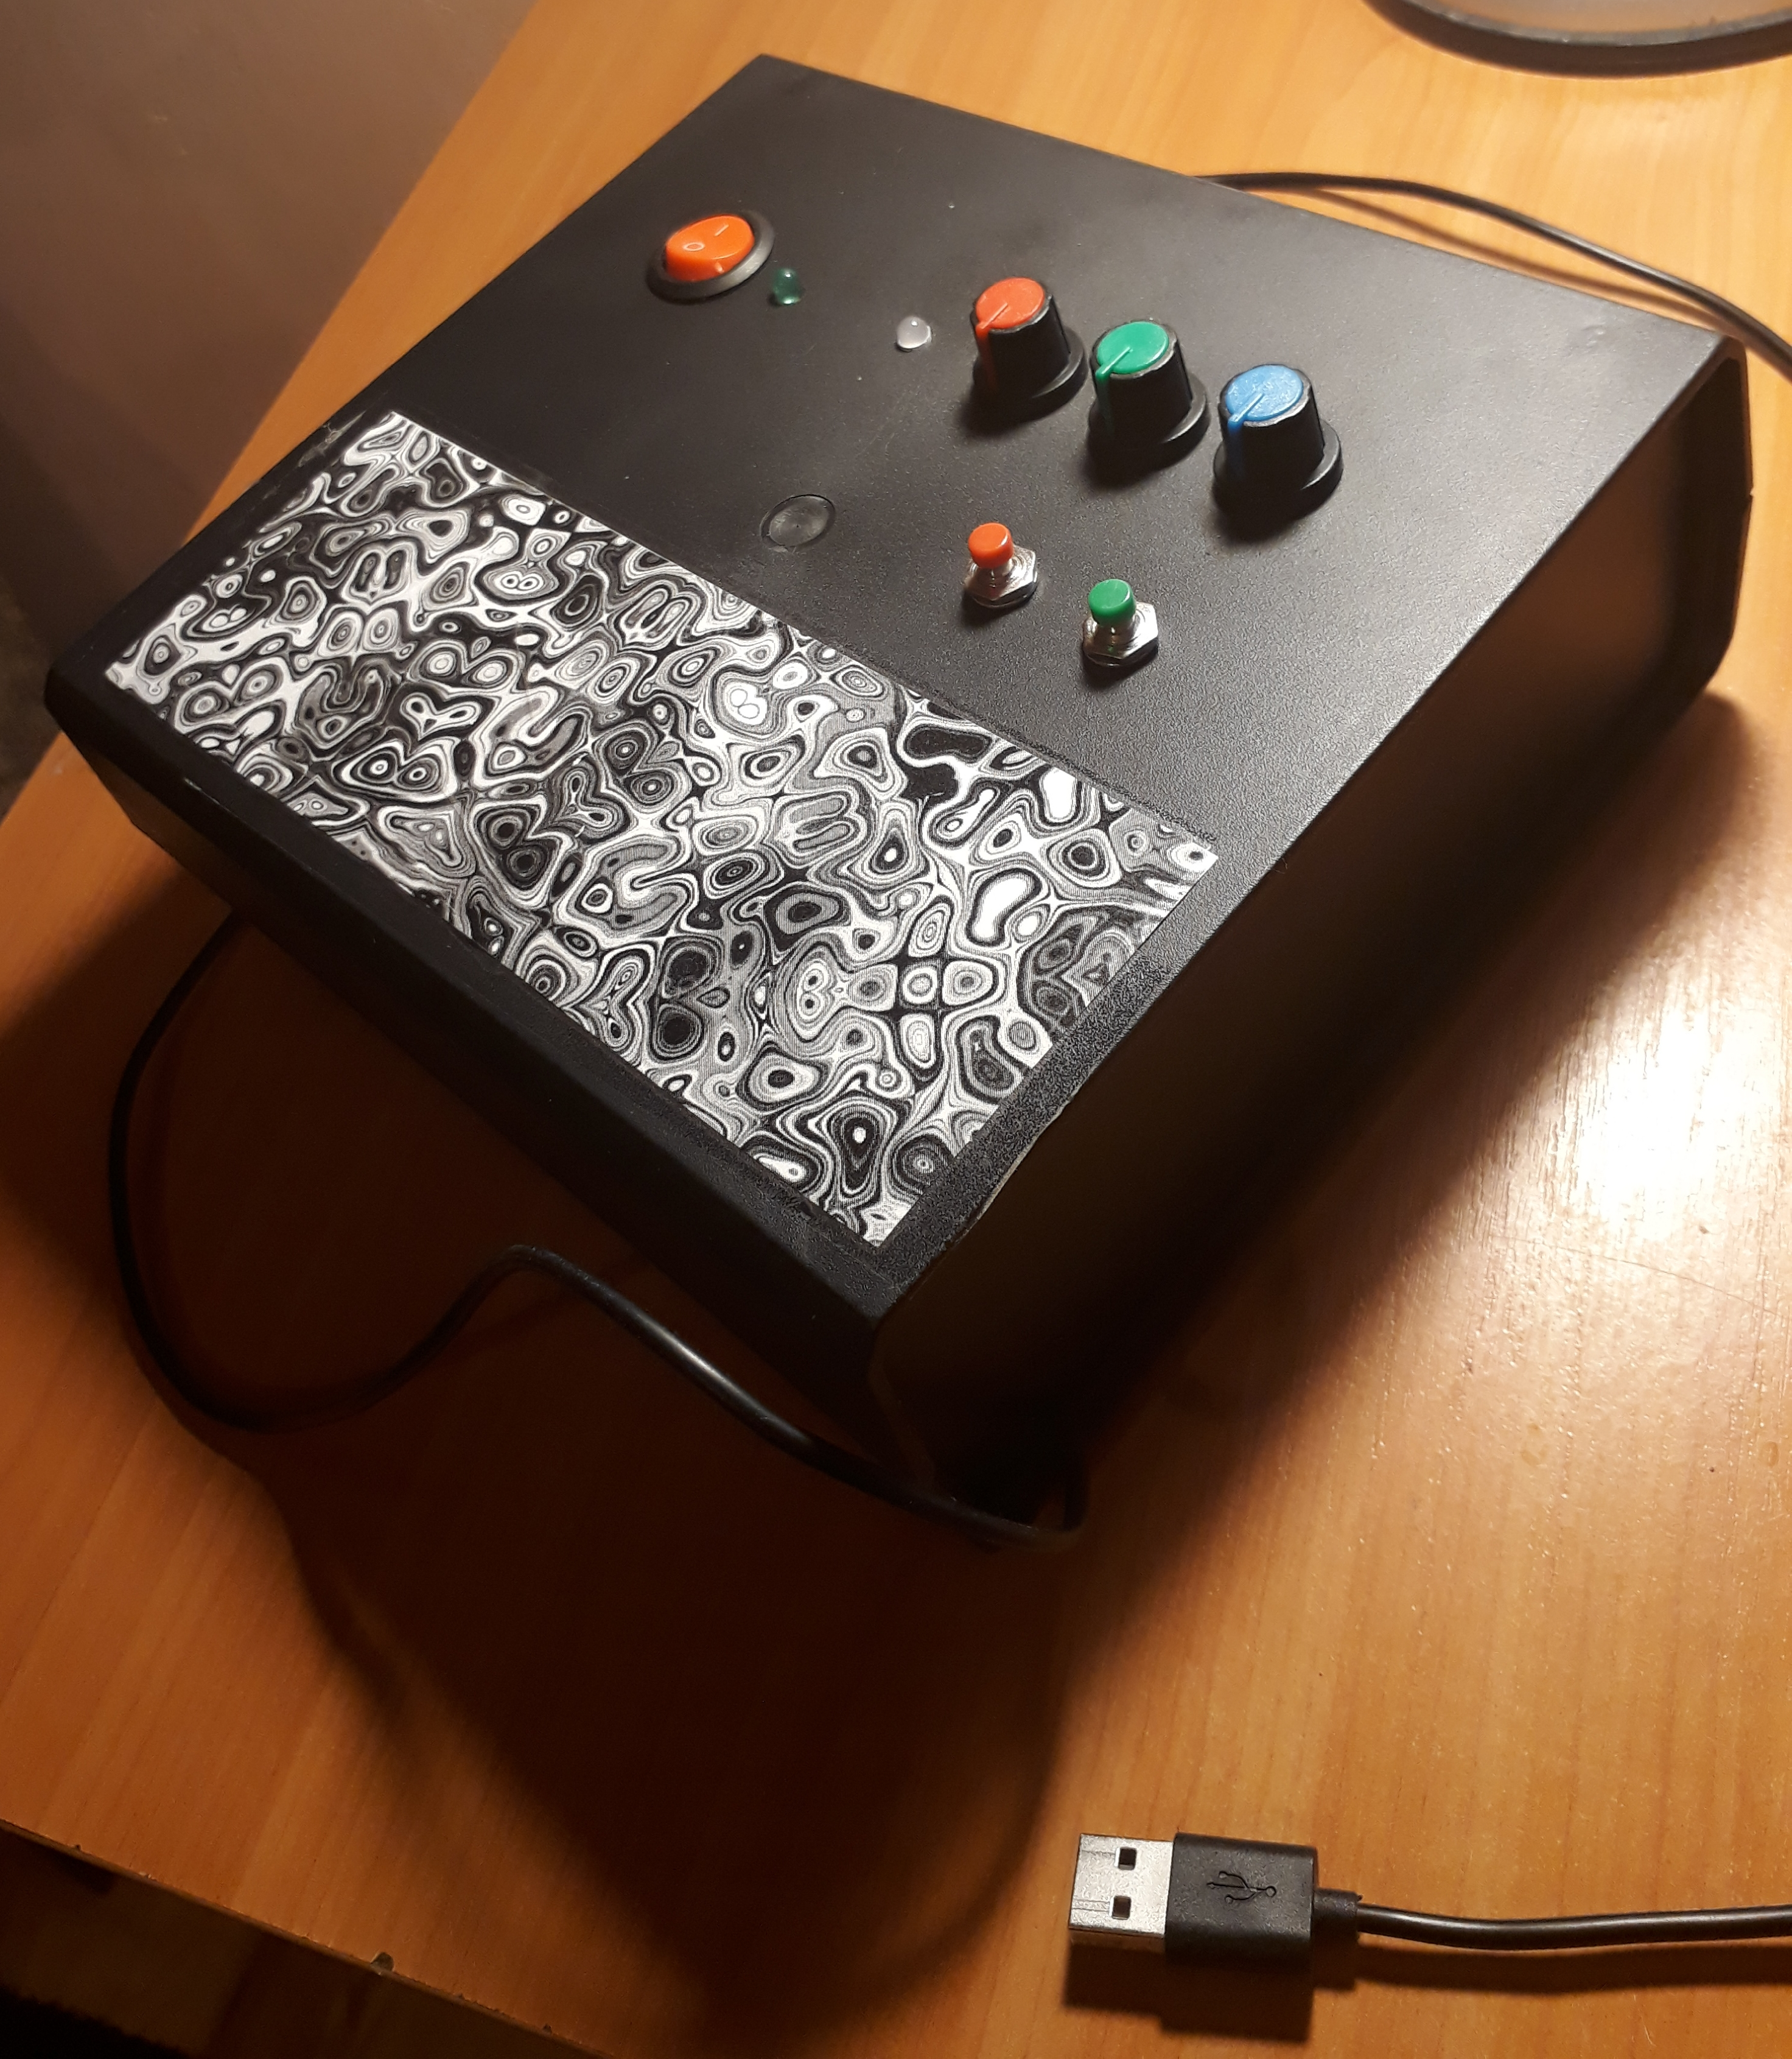
\includegraphics[width=0.6\textwidth]{device}
	\caption{Zdjęcie urządzenia. Źródło własne}
	\label{device}
\end{figure}

\subsubsection*{Schemat połączeń}
\begin{figure}[h]
	\centering	
	\includegraphics[width=\textwidth]{scheme2}
	\caption{Schemat połączeń. Źródło własne}
	\label{scheme}
\end{figure}


\begin{enumerate}[label=\alph*), leftmargin=1.25cm]
	\item A3, A4, A5 służą jako przetworniki analogowo/cyfrowe z rozdzielczością 1024. Ich zadaniem jest przetworzenie aktualnego stanu napięcia (rezystancji) na potencjometrach do wartości całkowitej w programie. Każdy z potencjometrów odpowiada za jedną składową koloru diody RGB. Kolejno R, G i B.
	\item D3, D5, D6 generują sygnał PWM doprowadzany do pinów diody RGB, kolejno R, G, B. Wartość wypełnienia zależy od stanu napięcia na potencjometrach.
	\item Przycisk na pinie 5V miał symulować przycisk włączenie/wyłączenia urządzenia, jednak ze względu na problemy w działaniu płytki Arduino po zmianie stanu, nie pełni on żadnej roli.
	\item Piny RX/TX zostały skrosowane i połączone z układem ESP8266.
	\item Dioda LED2 połączona do pinu D2 ma symbolizować uruchomienie układu.
	\item Przyciski połączone do pinów D8,D9 mają symulować zdarzenia , które pojawiły się w trakcie działania maszyny.
	\item Piny VCC oraz CH\_PD zostały połączone do źródłą zasilania z Arduino.
\end{enumerate}

\subsubsection*{Struktura plików}

Programy zawarte są w folderze arduino, w którym są 2 podfoldery: mqtt oraz mqtt\_tel, a każdy z nich zawiera po jednym pliku .ino. Wynika to z architektury Arduino, gdzie każdy skrypt powinien znajdować się w folderze o takiej samej nazwie. Oba pliki .ino zawierają analogiczny kod do mikrokontrolera, przy czym wariant z sufiksem \_tel posiada dane do logowania do sieci WiFi udostępnianej przez telefon autora, a skrypt bez sufiksu - do sieci lokalnej w domu autora.

\begin{figure}[h]
	\centering	
	\includegraphics[width=0.4\textwidth]{dirs_arduino}
	\caption{Struktura plików na urządzenie Arduino. Źródło własne}
\end{figure}

\subsubsection*{Omówienie programu}
Każdy program pisany dla Arduino można podzielić na trzy sekcje:
\begin{enumerate}[label=\alph*), leftmargin=1.25cm]
	\item importowanie bibliotek, definiowanie stałych i zmiennych,
	\item funkcja setup,
	\item funkcja loop.
\end{enumerate}

Zawartość pierwszej sekcji dokładnie opisuje punkt a) powyższej listy. Do zrealizowania projektu wykorzystano 3 biblioteki: WiFiESP - umożliwiające połączenie się z siecią WIFI poprzez układ ESP8266; PubSubClient - pozwala na publikowanie wiadomości protokołem MQTT; Bounce2 odpowiada za zredukowanie wpływu drgania styków w momencie wciśnięcia przycisku pushbutton. Tworzony jest tutaj także klient MQTT. Stałe definiować można na 2 sposoby, poprzez
\begin{lstlisting}
#define <nazwa> <wartosc>
\end{lstlisting}
co pozwala na bezpośrednie podmienienie nazwy w programie na wartość, bądź
\begin{lstlisting}
const <typ> <nazwa> = <wartosc>
\end{lstlisting}
Drugi sposób łączy nazwę zmiennej z komórką w pamięci podręcznej urządzenia, do której później program będzie się odwoływał gdy natrafi na daną nazwę. W programie występują również zmienne, definiowane w następujący sposób (fragment w nawiasach kwadratowych jest opcjonalny)
\begin{lstlisting}
<typ> nazwa [= <domyslna wartosc>];
\end{lstlisting}

% biblioteki, define, const, int, pubsubclient

Funkcja setup ma za zadanie przygotować program do późniejszego zadania. W tym miejscu ustawia się, czy pin ma pełnić funkcję wejścia czy wyjścia, konfiguruje się porty szeregowe, a także inicjuje połączenie wifi.

% połączenie wifi, ustawienei pinu, ustawienie seriala

Funkcja loop jest pętlą nieskończoną. Można z niej wyjść, natomiast spowoduje to przerwanie programu. W jej ciele wykonują się sczytania z pinów i ustawienie na nich wartości; wysyłane są również wiadomości do brokera MQTT. Wartości z potencjometrów domyślnie mieszczą się w zakresie 0-1023, natomiast na potrzeby programu, wartości te zostały przeskalowane do 0-255. Dodatkowo, w celu zwiększenia stabilności wartości, odczytane i przeskalowane wskazania są obniżane o 10, przy czym nie mogą być mniejsze od 0. Program zakłada, że broker jest informowany o zmianie wartości napięcia na potencjometrze tylko, jeśli obecna różni się o więcej niż 4 od ostatnio wysłanej. Publikowane jest wskazanie potencjometru przeskalowane do wartości 0-255. Wynika to z niedokładności przetwornika analogowo-cyfrowego, co nawet przy braku ingerencji we wskazania potencjometrów może doprowadzić do kaskady publikowanych wiadomości, co jest szumem komunikacyjnym. W celu redukcji wpływu drgań styków, odczytanie ostatecznej wartości na przycisku dokonuje się z opóźnieniem 50ms względem momentu wciśnięcia. Broker informowany jest jedynie, że przycisk został wysłany.

% screen połączenia się z wifi
% przykładowe odczytanie wartości rezystora, kliknięcie przycisku, ustawienie led, wysłanie msg
% powiedzieć o testamencie.


\subsection{System AR}
\subsubsection*{O systemie}
Przez system AR rozumie się zestaw współpracujących ze sobą skryptów napisanych w języku Python, który po włączeniu pobierze obraz z wybranego źródła i wyświetli zmodyfikowany obraz. Wszystkie pliki potrzebne do uruchomienia systemu znajdują się w folderze AR (rysunek \ref{dirs_ar_ref}). 

\begin{figure}[h]
	\centering
	\includegraphics[width=0.4\textwidth]{dirs_ar}
	\caption{Struktura plików w projekcie. Źródło własne}
	\label{dirs_ar_ref}
\end{figure}

Poza skryptami, których dokładny opis i wyjaśnienie działania przedstawione zostaną w kolejnym podrozdziale, w tej samej lokalizacji znajduje się folder z plikiem konfiguracyjnym, oraz obrazkami. Konfiguracja napisana została w pliku JSON, jej uproszczoną zawartość prezentuje Listing \ref{ar_config}.

\begin{lstlisting}[language=json,firstnumber=1,caption=Plik konfiguracyjny użyty w projekcie, label=ar_config]
{
	"server": {
		"protocol": "mqtt",
		"host": "localhost",
		"port": 1883,
		"topics": [
		{
			"topic": "arduino/red",
			"name": "red",
			"default": 0,
			"type": "int"
		},
		{...}]
	},
	"machines": [
		{
		"name": "Test Machine",
		"ref": "img/base.png",
		"areas": {
			"PB": [92, 144, 178, 233],
			(...)
		}}
	]
}
\end{lstlisting}

Wydzielone zostały 2 główne sekcje:

\begin{enumerate}[label=\alph*), leftmargin=1.25cm]
	\item server - zawiera informacje wymagane do połączenia z brokerem MQTT, takie jak adres hosta, port, oraz listę tematów, które powinny być nasłuchiwane. Każdy temat reprezentuje jedna tablica asocjasyjna, zawierające klucze dotyczące nazwy tematu po stronie mqtt, nazwy tematu po stronie aplikacji, oraz opcjonalnie domyślnej wartości i typu, na który powinna zostać przekonwertowana zmienna po odbiorze.
	\item machines - lista maszyn, które algorytm będzie próbował znaleźć. W chwili pisania niniejszej pracy algorytm jest dostosowany do rozpoznawania jedynie jednej maszyny, ale pozostawiono furtkę do późniejszego rozwinięcia. Każda maszyna w konfiguracji to tablica asocjacyjna, która zawiera nazwę maszyny, ścieżkę do obrazka referencyjnego, oraz listę par klucz-wartość, reprezentującą potencjalnie interesujące obszary na panelu maszyny. Para ma strukturę: <nazwa\_obszaru>: [x1, y1, x2, y2], gdzie wartości są parami współrzędnych kartezjańskich wyznaczonych z obrazu referencyjnego.
\end{enumerate}

\subsubsection*{Obraz referencyjny}

Obrazem referencyjnym użytym w projekcie jest zdjęcie panelu urządzenia testowego, zrobionego za pomocą kamery webcam użytej do późniejszego testowania systemu. Rysunek \ref{base_img} przedstawia tenże obraz, a \ref{base_img_kp} wyznaczone z niego punkty charakterystyczne. Zauważyć można, że elementy użytkowe panelu nie pozwalają na wyznaczenie dużej liczby punktów, z tego też powodu do dolnej części panelu przyklejono wzór, który pozwala zauważalnie zwiększyć stabilność rozpoznawania.
\begin{figure}[h]
	\centering
	\includegraphics[width=0.6\textwidth]{base}
	\caption{Obraz referencyjny. Źródło własne}
	\label{base_img}
\end{figure}
\begin{figure}[h]
	\centering
	\includegraphics[width=0.6\textwidth]{base_kp}
	\caption{Obraz referencyjny. Źródło własne}
	\label{base_img_kp}
\end{figure}


\subsubsection*{Stworzone skrypty}
\textbf{main.py} - Główny skrypt systemu, w celu jest uruchomienia powinien zostać uruchomiony przez użytkownika. Dostępnymi parametrami są:
\begin{itemize}
	\item -t/--type - typ źródła strumienia wideo. Dostępne są: remote (po adresie IP), file (z pliku), cam (kamera połączona bezpośrednio z komputerem), image (pojedyncza klatka). Domyślną wartością jest cam.
	\item -s/--source - źródło strumienia, zależna od typu. Więc może to być kolejno: adres IP, ścieżka do pliku, id kamery, ścieżka do obrazka.
	\item -c/--config - ścieżka do pliku konfiguracyjnego. Domyślnie ../config/config.json.
\end{itemize}
W samym pliku znajduje się również skrypt inicjujący działanie systemu. Odbywa się to w kilku krokach. Na początku tworzony jest obiekt strumienia wideo cap. Następnie tworzona jest instancja systemu, przyjmująca konfigurację JSON jako argument. Opcjonalnymi krokami są: obrysowanie rozpoznanego obiektu, oraz wyświetlanie liczby klatek na sekundę (FPS). Kolejnym krokiem jest wywołanie metody add\_layer, w której parametrem jest funkcja modyfikująca obraz z kamery. Ostatnim krokiem jest wywołanie metody run, która zaczyna pobierać obraz ze strumienia i go odpowiednio przetwarzać. Schemat tego działania przedstawia Listing \ref{init_listing}.

\begin{lstlisting}[language=Python,caption=Uruchomienie systemu,label=init_listing]
# Parse CLI arguments
args = prepare_arguments()

# Setup VideoCapture
cap = Stream(args.source, args.type)

# Init AugumentAPI instance based on config
augument = AugumentAPI(args.config)
augument.outline_detection()
augument.show_fps()
augument.add_layer(draw_stats)

# Run 
augument.run(cap)
\end{lstlisting}

Funkcja rysująca przyjmuje trzy parametry. Pierwszym z nich jest frame, czyli obiekt klasy Frame, machine - tablica asocjacyjna z pliku konfiguracyjnego, oraz params - parametry z tematów MQTT. Funkcja ta musi zwrócić frame. Poniższy fragment (listing \ref{draw_fn}) rzeczywistej funkcji użytej w projekcie, ma za zadanie narysować biały prostokąt, oraz tekst "Urzadzenie wylaczone" w odpowiednim miejscu na kadrze jeśli parametr "connected" ma wartość "OFF". Docelowo funkcja rysująca jest jedynym miejscem, poza plikiem konfiguracyjnym, który późniejszy użytkownik powinien modyfikować. Funkcja rysująca wywoływana jest dla każdego kadru.

\begin{lstlisting}[language=Python,caption=Uruchomienie systemu,label=draw_fn]
if params["connected"] == "OFF":
	frame.draw_rectangle((10, 30), (170,37))
	frame.draw_text("Urzadzenie wylaczone", (20, 50))
\end{lstlisting}

\textbf{Stream.py}
Skrypt zawiera klasę Stream, która tworzy instancję obiektu strumienia video, który zostanie później użyty w projekcie. W zależności typu źródła podanego w parametrach głównego skryptu main.py, obiekt się delikatnie różni, jednak każdy wariant posiada metody: cap, release, read, aby cały system mógł działać poprawnie. Dodatkowo w przypadku wariantu z kamerą połączoną bezpośrednio z komputerem, skrypt ustawia odpowiednią rozdzielczość, oby ograniczyć zużycie zasobów. Klasa Stream przyjmuje 2 parametry w swojej funkcji inicjującej: source oraz source\_type, które odpowiadają parametrom --source i --type.


\textbf{Store.py}
Zawiera definicję klasy Store, której zadaniem jest nadzorowanie stanu parametrów przekazywanych przez MQTT. Zawiera metody pozwalające na zmapowanie nazwy tematu na nazwę parametru w aplikacji, pobranie i ustawienie stanu. Funkcja inicjująca przyjmuje listę tematów z pliku konfiguracyjnego. Stan to tablica asocjacyjna zawierająca pary parametr-wartość. Listing \ref{store} przedstawia proces stworzenia i ustawienie wartości dla parametru "test"

\begin{lstlisting}[language=Python,label=store,caption=Uruchomienie systemu]
topics = [{"topic": "test/topic", "name": "top", "default": 0}]
store = Store(topics) # {"top": 0}

store.set_state("top", 100)
store.get_state() # {"top": 100}
\end{lstlisting}

\textbf{Machine.py}
Plik Machine.py zawiera klasę o tej samej nazwie. Jest to prosta klasa zawierająca w sobie informacje na temat pojedynczej maszyny: nazwę, obraz referencyjny oraz listę obszarów. Klasa zawiera pole statyczne all, pozwalające na śledzenie stanu rozpoznawanych maszyn. Zawiera publiczną metodę get\_area, która na podstawie nazwy obszaru zwróci jego współrzędne, a w razie potrzeby wywoła wyjątek. Posiada też pola name, areas i ref\_image, zawierające informacje o obiekcie. Listing \ref{mach} pokazuje proces tworzenia instancji klasy, jak i pobierania obszaru.

\begin{lstlisting}[language=Python,label=mach, caption=Stworzenie instancji Machine]
config = {"name": "Maszyna", "ref": "test.jpg", "areas":{"A1": [0,0,100,100]}}
machine = Machine(config)

machine.get_area("A1") # [0,0,100,100]
machine.get_area("Void")
# Traceback (most recent call last):
#   File "<stdin>", line 1, in <module>
#   File "/home/rafcio/Mgr/AR/Machine.py", line 28, in get_area
#     raise ValueError("No area named" + label)
# ValueError: No area named VOID 
\end{lstlisting}

\textbf{Detector.py}
Detektor.py zawiera klasę Detector. Jej zadaniem jest znalezienie homografii pomiędzy obrazkiem referencyjnym, a kadrem z kamery. W ramach inicjującej przyjmowana jest struktura maszyny. Po pobraniu obrazka referencyjnego, tworzony jest deskryptor, domyślnie ORB, ustawiony na wykrywanie 1000 punktów kluczowych. \textbf{SPRAWDZIĆ}. Następnie za jego pomocą wyznaczane są punkty kluczowy oraz deskryptory obrazu referencyjnego, oraz przygotowywany jest matcher FLANN. Całość tego procesu przedstawia Listing \ref{detecotor}

\begin{lstlisting}[language=Python,label=machine,caption=Stworzenie instancji Detector]
class Detector(object):
	def __init__(self, machine):
		self.__machine = machine

		# Reference image
		ref_img = cv2.imread(machine["ref"])
		self.__ref_image = ref_img
		
		# Prepare descriptor
		self.__descriptor = cv2.ORB_create(1000)
		
		# Compute keypoints and descriptors for reference image
		self.__kp, self.__desc = self.detectAndCompute(self.__ref_image)

		# Prepare matcher
		self.__index_params = dict(algorithm = 6,           # FLANN_INDEX_LSH
							       table_number = 12,
								   key_size = 20,
								   multi_probe_level = 1)
		self.__search_params = dict(checks=300)
		self.__matcher = cv2.FlannBasedMatcher(self.__index_params, self.__search_params)
\end{lstlisting}

Klasa zawiera statyczne metody: calc\_good\_points, która filtruje znalezione dopasowania, oraz false\_detection, zwracającą krotkę charakterystyczną dla braku detekcji obiektu na obrazie. Publiczne metody to detect, przyjmująca kadr z kamery, a zwracająca wartość boolowską czy znaleziono, macierz homografii oraz maskę; get\_pts, zwracająca macierz zawierającą współrzędne narożników obrazka referencyjnego. Jest to przydatne podczas rysowania zgodnego z perspektywą urządzenia.

\textbf{Client.py}
Plik zawiera klasę ClientMQTT, umożliwiającą sprawną komunikację z brokerem. Funkcja inicjująca posiada dwa opcjonalne argumenty: host oraz port. W przypadku ich braku domyślnymi wartościami są kolejno "localhost" i 1883. Klasa umożliwia dodanie własnych wywołań zwrotnych (ang. callback) dla połączenia i rozłączenie z brokerem, w przypadku nowej wiadomości od brokera. Kluczową dla działania systemu jest metoda register\_handler, która przyjmuje nazwę tematu oraz funkcję zwrotną, wywoływaną, gdy przyjdzie nowa wiadomość z podanego tematu. Callback przyjmuje nazwę eventu oraz samą wiadomość. Handlery są dodawane automatycznie dla każdego topicu, dzięki czemu możliwa jest aktualizacja stanu aplikacji w czasie rzeczywistym.

\begin{lstlisting}[language=Python, caption=Tworzenie instancji klienta]
def handler(event, msg):
	fn("New message on {} topic: {}".format(event, msg))

client = ClientMQTT(host="localhost", port=1883)

cient.register_handler("topic", handler)
client.connect()
\end{lstlisting}

\textbf{DrawAPI.py}
Plik zawiera:

\begin{enumerate}[label=\alph*), leftmargin=1.25cm]
\item Klasę T - zawiera typy możliwych transformacji na metodzie rysującej. W chwili obecnej są to: FOLLOW - nakładka na kadr nie jest transformowana geometrycznie, ale początek jej lokalnego układu współrzędnych (lewy góry narożnik) podąża za początkiem układu współrzędnych rozpoznanego obiektu; PERSPECTIVE - na nakładkę aplikowana jest homografia, przez co ma ona wspólną płaszczyznę z panelem urządzenia.

\begin{lstlisting}[language=Python]
class T:
	"""Transform types"""
	FOLLOW=0
	PERSPECTIVE=2
\end{lstlisting}

\item Klasę Frame - semantycznie jest to obiekt kadru z kamery. W ramach inicjalizacji konieczne jest podanie obrazu, natomiast opcjonalnymi parametrami są: macierz homografii, maska homografii, oraz rozmiar obrazu referencyjnego.

Klasa Frame udostępnia metody:

\item draw\_rectangle - rysuje prostokąt o zadanym: początku, rozmiarze, kolorze oraz transformacji. Domyślnie prostokąt jest biały oraz bez transformacji. Reszta parametrów jest obligatoryjna. Przykład:
\begin{lstlisting}[language=Python]
draw_rectangle((100,100), (50, 90), color=(255, 0, 0), transform=T.PERSPECTIVE)
\end{lstlisting}
\begin{figure}[h]
	\centering
	\includegraphics[width=0.5\textwidth]{draw_rect}
	\caption{Rysowanie prostokąta. Źródło własne}
\end{figure}

\item draw\_polylines - rysuje wielokąt. Wymaganym parametrem jest lista krotek dwuelementowych, zawierająca współrzędne kolejnych wierzchołków. Opcjonalnymi parametrami są: kolor oraz grubość linii. Przykład:
\begin{lstlisting}[language=Python]
frame.draw_polylines([np.int32([(10,10),(30, 40), (70, 20), (90,100)])], color=(0, 255, 0))
\end{lstlisting}
\begin{figure}[h]
	\centering
	\includegraphics[width=0.3\textwidth]{draw_poly}
	\caption{Rysowanie wielokąta. Źródło własne}
\end{figure}

\item draw\_text - rysuje na kadrze tekst o zadanej treści i współrzędnych. Wśród opcjonalnych parametrów są: krój fontu, rozmiar, kolor, grubość linii, sposób wygładzania linii  oraz sposób transformacji. Przykład:
\begin{lstlisting}[language=Python]
frame.draw_text("img/rot_arr_cw.png", (20, 50), size=0.5)
\end{lstlisting}
\begin{figure}[h]
	\centering
	\includegraphics[width=0.5\textwidth]{draw_text}
	\caption{Rysowanie tekstu. Źródło własne}
\end{figure}

\item draw\_image - rysunek inny obrazek. Konieczne jest podanie drugiej obrazu, natomiast opcjonalne są: współrzędne (domyślnie punkt (0,0)), rozmiar (domyślnie rozmiar obrazka) oraz sposób transformacji. Przykład:
\begin{lstlisting}[language=Python]
frame.draw_image(path, (160, 400), (50, 50), transform=T.PERSPECTIVE)
\end{lstlisting}
\begin{figure}[h]
	\centering
	\includegraphics[width=0.5\textwidth]{draw_img}
	\caption {Rysowanie obrazka. Źródło własne}
\end{figure}

\item get\_image - bezparametrowa funkcja zwracająca aktualny kadr, razem z ewentualnymi zmianami.
\end{enumerate}

Dzięki temu, że każda z wymienionych metod zwraca całą instancję, możliwe jest wywołań i pisanie kodu w postaci:
\begin{lstlisting}[language=Python]
frame \
	.draw_rectangle((10,10),(100,100), color=(255,255,0)) \
	.draw_text("TEST", (30, 30))
\end{lstlisting}
Co skutkuje narysowaniem na ekranie
\begin{figure}[h]
	\centering
	\includegraphics[width=0.5\textwidth]{chaining}
	\caption{Rysowanie prostokąta i tekstu. Źródło własne}
\end{figure}


\textbf{AugumentAPI.py}
Zawarta w pliku klasa AugumentAPI jest jedną z 2 obiektów, które powinny zostać zainicjowane w skrypcie głównym main.py. Pierwszym z nich jest obiekt strumienia video, a drugim właśnie AugumentAPI, które ten właśnie strumień przyjmie w funkcji startu run. Dodatkowo podczas inicjalizacji obiektu należy podać ścieżkę do pliku konfiguracyjnego w formacie json, co przedstawia listing \ref{aug}.

\begin{lstlisting}[language=Python, label=aug, caption=Tworzenie oraz uruchomienie systemu AR]
augument = AugumentAPI(config)
augument.run(cap)
\end{lstlisting}

W ramach inicjalizacji skonfigurowane zostaną obiekty Detector, Client oraz Store, oraz zasubskrybowane będą tematy MQTT pobrane z pliku konfiguracyjnego. Klasa zawiera metodę add\_layer, w ramach której podaje się funkcję rysującą. Zostaje ona do pola \_\_layers. Wykorzystane jest ono w metodzie parse\_frame w ramach której na kadr nakładane są elementy stworzone w funkcji rysujących. Ponieważ wywoływanie podanych funkcji jest realizowane w ramach kolejki FIFO, możliwe jest tworzenie warstw jedna na drugiej. Może to być szczególnie pomocne podczas tworzenia bardziej skomplikowanych interfejsów.

Inne dostępne dla użytkownika metody to:
\begin{enumerate}[label=\alph*), leftmargin=1.25cm]
	\item stop() - zatrzymuje działanie systemu
	\item show\_fps() - pokazuje klatkaż w lewym górnym rogu ekranu
	\item outline\_detection() - rozpoznany obiekt zostaje obrysowany czerwoną linią
\end{enumerate}

\textbf{util.py}
Zawiera dodatkowe generyczne funkcje wykorzystywane w każdym z plików projektu. Zawiera między innymi metody na wyświetlanie informacji w terminalu w zależności od ich przeznaczenia: info, warning, error, success; przeskaluj obraz, aby jego rozmiar nie przekraczał maksymalnego, bez zmiany skali, odczytaj plik JSON i inne.


\subsection{Komunikacja}
Komunikacja odbywa się za pomocą protokołu MQTT, którego opis przedstawiono w jednym z poprzednich rozdziałów. Aby założenia projektowe mogły być spełniono, wyznaczono tematy do komunikacji
\begin{enumerate}
	\item connected - temat informujący czy urządzenie ma aktywne połączenie z brokerem. Może przyjąć wartość "ON" bądź "OFF". Jest to specjalny kanał, ponieważ dzięki zastosowaniu techniki "testamentu", 5 sekund po przerwaniu połączenia z brokerem, temat przyjmie wartość "OFF".
	\item arduino/red - zawiera składową czerwonego koloru. Przyjmuje wartości o 0 do 255 typu String. Jest to wartość potencjometrze na rezystorze R1, z czerwoną gałką.
	\item arduino/green - zawiera składową zielonego koloru. Przyjmuje wartości o 0 do 255 typu String. Jest to wartość potencjometrze na rezystorze R2, z zieloną gałką.
	\item arduino/blue - zawiera składową niebieskiego koloru. Przyjmuje wartości o 0 do 255 typu String. Jest to wartość potencjometrze na rezystorze R3, z niebieską gałką.
	\item arduino/mode - przyjmuje wartości od 0 do 2 typu String. Oznacza tryb, opisany w następnym podrozdziale. Wartość jest zwiększa o 1, bądź ustawiania na 0 po wciśnięciu przycisku B1.
\end{enumerate}

\subsection{Tryby działania}
W celu przeprowadzenia prezentacji, autor podjął decyzję o stworzeniu 3 trybów pokazowych, mających zademonstrować działanie systemu.

Pierwszym trybem jest tryb pokazowy. Za pomocą strzałek oznaczone są wszystkie obszaru opisane w pliku konfiguracyjnym dla każdej maszyny. Na strzałki nałożona jest homografia, wobec czego podążają one za obszarami oraz są one transformowane geometrycznie. Dodatkowo w lewym górnym narożniku ekranu rysowany jest obszar informacyjny, z wartościami liczbowymi składowych kolorów, a także aktualnym trybem.


\begin{figure}[h]
	\centering
	\includegraphics[width=0.5\textwidth]{pres}
	\caption{Tryb prezentacji. Źródło własne}
\end{figure}

Drugi i trzeci tryb mają analogiczne działanie. Otóż celem tego trybu jest pokierowanie użytkownika tak, aby dioda RGB świeciła na odpowiedni kolor. Składowe dla trybu drugiego (limonkowy) to (100, 200, 0), kolejno dla koloru czerwonego, zielonego i niebieskiego. Trzeci tryb nazwany został turkusowym, a pożądane składowe to (5, 85, 35). Ze względu na niedokładność potencjometrów i przetwornika analogowo/cyfrowego Arduino, przyjęto dokładność +/- 15. W przypadku, gdy dana składowa nie mieści się w pożądanym obszarze, na obrazie rysowana jest strzałka skierowana w kierunku, w którym gałka potencjometru powinna zostać obrócona. Obrazuje to rysunek \ref{limref}

\begin{figure}[h]
	\centering
	\includegraphics[width=0.5\textwidth]{lim}
	\caption{Tryb limonkowy. Źródło własne}
	\label{limref}
\end{figure}



\section{Testy}
W celu ustalenia sprawności i dokładności systemu rozpoznawania obiektu, autor podjął decyzję o wykonaniu testów dla różnych warunków. Testy, nie licząc testu odległości, wykonano w odległości 50cm kamery od urządzenia. Wykorzystana została kamera internetowa Tecknet c018 FullHD oraz lampa symulująca różne warunki oświetleniowe.  Stanowisko testowe zostało przedstawione na rysunku \ref{test_station}

Testy wykonano poprzez zwiększanie bądź zmniejszanie badanego parametru do momentu, w którym rozpoznawanie było stabilne. Każdy z punktów brzegowych został uwieczniony i przedstawiony w stosownym podrozdziale w postaci zdjęcia sytuacji.

\begin{figure}[h]
	\centering
	\includegraphics[width=0.5\textwidth]{test_stat}
	\caption{Stanowisko do testów. Źródło własne}
	\label{test_station}
\end{figure}

Wykonane zostały:
\begin{enumerate}[label=\alph*), leftmargin=1.25cm]
\item Test odległości
\item Test kąta patrzenia
\item Test różnych warunków oświetleniowych
\item Test różnego natężenia oświetlenia
\item Test obrotu kamery względem urządzenia
\item Test częściowo widocznego urządzenia
\end{enumerate}

\subsection{Test odległości}
Testowano poprzez przesuwanie kamery wzdłuż osi głównej ustawionej prostopadle do płaszczyzny panelu urządzenia. Rozpoznawanie było stabilne w zakresie 10-90cm. W przypadku bliższego wariantu, fakt czy urządzenie zostało rozpoznane zależało od obecności wzoru na kadrze - jego brak powodował brak detekcji, patrz rys. \ref{test_close1}.
\begin{figure}[htb!]
	\begin{subfigure}[b]{0.5\textwidth}
		\includegraphics[width=\textwidth]{test_close1}
		\caption{10cm, bez wzoru}
		\label{test_close1}
	\end{subfigure}
	\begin{subfigure}[b]{0.5\textwidth}
		\includegraphics[width=\textwidth]{test_close2}
		\caption{10cm, ze wzorem}
		\label{test_close2}
	\end{subfigure}
	\begin{subfigure}[b]{0.5\textwidth}
		\includegraphics[width=\textwidth]{test_close3}
		\caption{90cm}
		\label{test_close3}
	\end{subfigure}
	\caption{Testy odległości. Źródło własne}
\end{figure}
\FloatBarrier


\subsection{Test kąta patrzenia}
Testy wykonano dla różnych katów pomiędzy osią główną kamery, a płaszczyzną panelu urządzenia, dla odległości 50cm. Wykonane próby dowiodły, że urządzenie jest poprawnie wykrywane do odchylenia około 45 stopni w dowolnej płaszczyźnie (rys. \ref{test_angl1}, \ref{test_angl2}).

\begin{figure}[htb!]
	\begin{subfigure}{0.5\textwidth}
		\includegraphics[width=\textwidth]{test_angle1}
		\caption{45\degree w płaszczyźnie poziomej}
		\label{test_angl1}
	\end{subfigure}
	\begin{subfigure}{0.5\textwidth}
		\includegraphics[width=\textwidth]{test_angle2}
		\caption{45\degree w płaszczyźnie pionowej}
		\label{test_angl2}
	\end{subfigure}
	\caption{Test kąta patrzenia. Źródło własne}
\end{figure}
\FloatBarrier

\subsection{Test różnych warunków oświetleniowych}
Poprzez warunki oświetleniowe rozumie się punktowe źródło światła skierowane z boku urządzenia. Celem było sprawdzenie, czy cienie rzucane przez wypukłe elementy panelu wpływają na detekcje.
\begin{figure}[htb!]
	\begin{subfigure}{0.46\textwidth}
		\includegraphics[width=\textwidth]{test_light1}
		\caption{na wprost}
		\label{test_light1}
	\end{subfigure}
	\begin{subfigure}{0.46\textwidth}
		\includegraphics[width=\textwidth]{test_light2}
		\caption{z boku}
		\label{test_light2}
	\end{subfigure}
	\begin{subfigure}{0.46\textwidth}
		\includegraphics[width=\textwidth]{test_light3}
		\caption{od góry}
		\label{test_light3}
	\end{subfigure}
	\caption{Test różnych warunków oświetleniowych. Źródło własne}
\end{figure}
\FloatBarrier


\subsection{Test różnego natężenia oświetlenia}
Celem testu było sprawdzenie jak system detekcji działa w warunkach słabego oświetlenia. Detekcje były poprawne średniego i słabego oświetlenia (rys. \ref{test_bright1}, \ref{test_bright2}). Dla oświetlenia bardzo słabego, czyli takiego dla którego elementy panelu nie były już wyraźnie, detekcja nie następowała (rys. \ref{test_bright3}).
\begin{figure}[htb!]
	\begin{subfigure}[b]{0.5\textwidth}
		\includegraphics[width=\textwidth]{test_bright1}
		\caption{średnie oświetlenie}
		\label{test_bright1}
	\end{subfigure}
	\begin{subfigure}[b]{0.5\textwidth}
		\includegraphics[width=\textwidth]{test_bright3}
		\caption{słabe oświetlenie}
		\label{test_bright2}
	\end{subfigure}
	\begin{subfigure}[b]{0.5\textwidth}
		\includegraphics[width=\textwidth]{test_bright2}
		\caption{bardzo słabe oświetlenie}
		\label{test_bright3}
	\end{subfigure}
	\caption{Test różnych natężeń oświetlenia. Źródło własne}
\end{figure}
\FloatBarrier

\subsection{Test obrotu kamery względem urządzenia}
Celem było sprawdzenie jak detekcja reaguje na obrót obrazu względem osi głównej kamery. Testowano poprzez obracanie kamery co 90\degree.

\begin{figure}[htb!]
	\begin{subfigure}[b]{0.5\textwidth}
		\includegraphics[width=\textwidth]{test_rot1}
		\caption{90\degree w prawo}
		\label{test_rot1}
	\end{subfigure}
	\begin{subfigure}[b]{0.5\textwidth}
		\includegraphics[width=\textwidth]{test_rot2}
		\caption{180\degree}
		\label{test_rot2}
	\end{subfigure}
	\begin{subfigure}[b]{0.5\textwidth}
		\includegraphics[width=\textwidth]{test_rot3}
		\caption{90\degree w lewo}
		\label{test_rot3}
	\end{subfigure}
	\caption{Test obrotu względem osi głównej kamery. Źródło własne}
\end{figure}
\FloatBarrier


\subsection{Test częściowo widocznego urządzenia}
Celem było przetestowanie zachowania algorytmu detekcji dla częściowo zasłoniętego panelu urządzenia. Wykonano łącznie pięć testów: dwa symulujące naturalne zachowania, to jest ludzka dłoń korzystająca z panelu, trzeci testował zachowanie przy niewidocznym wzorze, a dwa ostatnie sprawdzały procentowe zasłonięcie panelu.

Gdy cześć panelu została zasłonięta dłonią, detekcja była poprawna. W przypadku, gdy całość wzoru nie była widoczna, detekcja nie następowała. Dla dwóch ostatnich pomiarów, urządzenie było rozpoznawane jeśli conajmniej 25\%-50\% było widoczne.

\begin{figure}[htb!]
	\begin{subfigure}[b]{0.5\textwidth}
		\includegraphics[width=\textwidth]{test_cover1}
		\caption{90\degree w prawo}
		\label{test_cover1}
	\end{subfigure}
	\begin{subfigure}[b]{0.5\textwidth}
		\includegraphics[width=\textwidth]{test_cover2}
		\caption{180\degree}
		\label{test_cover2}
	\end{subfigure}
	\begin{subfigure}[b]{0.5\textwidth}
		\includegraphics[width=\textwidth]{test_cover3}
		\caption{90\degree w lewo}
		\label{test_cover3}
	\end{subfigure}
	\begin{subfigure}[b]{0.5\textwidth}
		\includegraphics[width=\textwidth]{test_cover4}
		\caption{180\degree}
		\label{test_cover4}
	\end{subfigure}
	\begin{subfigure}[b]{0.5\textwidth}
		\includegraphics[width=\textwidth]{test_cover5}
		\caption{90\degree w lewo}
		\label{test_cover5}
	\end{subfigure}
	\caption{Test częściowo widocznego urządzenia. Źródło własne}
\end{figure}
\FloatBarrier

\subsection{Podsumowanie i wnioski z testów}
\begin{enumerate}[label=\alph*), leftmargin=1.25cm]
\item W teście odległości, maksymalną wartość zwiększyć można korzystając z lepszej kamery, bądź opierając się na obrazie w większej rozdzielczości
\item Wykorzystana kamera rozmazuje obraz w ruchu
\item Obrót względem osi głównej nie wpływa na poprawność detekcji
\item Urządzenie jest poprawnie rozpoznawane dla +/-45\degree w dowolnej osi, wydaje się to być wartością wystarczającą do praktycznego wykorzystania systemu
\item Rozpoznanie nie występuje dla bardzo słabego oświetlenia. Można to poprawić poprzez obróbkę obrazu przed detekcją, na przykład rozjaśnienie, bądź zwiększenie kontrastu, lub wykorzystanie lepszej kamery
\item Pozycja źródła światła (a więc cienie) nie wpływa na poprawność detekcji
\item Przy w większości zasłoniętym panelu występują problemy z rozpoznawaniem, szczególnie, gdy nie jest widoczny wzór. W praktyce, dla bardziej skomplikowanych panelów nie powinno być to aż tak uciążliwe, jednak poprawę sytuacji zapewni rozmieszczenie wzorów w różnych miejscach.
\end{enumerate}
\clearpage


\section{Podsumowanie i wnioski końcowe}
Wykorzystanie AR do celów użytkowania i obsługi urządzeń jest bez wątpienia przyszłością. Możliwości jakie zapewnia rozszerzenie widocznego obrazu pozwala na odciążenie pracowników, dzięki czemu będą oni popełniać mniej błędów, ponieważ niektóre decyzje podejmować może program. Dodatkowo ze względu na dostęp do danych w czasie rzeczywistym pozwala na przyspieszenie części zadań. Urządzenie stworzone na potrzeby pracy było w pełni zamknięte, nie posiadające zewnętrznych portów dostępowych, ani wyświetlaczy. Jest to w niektórych przypadkach wymagane, jeśli urządzenie jest podane na warunki zewnętrzne, a pracuje w takich warunkach. Wtedy dostęp do niektórych funkcji może być utrudniony, jednak wyświetlanie odpowiednich parametrów przed oczami pracownika rozwiązuje ten problem.

Tryby, w których pracownik jest prowadzony za rękę przez specjalnie przygotowany tryb, pokazujący kolejne kroki procesu pozwoli zredukować czas uczenia, a także koszty z tym związane. Zamiast wysyłać serwisanta lub trenera na miejsce usterki czy też treningu, nawiązać można wideo rozmowę, gdzie obaj będą widzieć ten sam obraz, co pozwala na bezproblemową komunikację.

Udało się wykonać projekt, który spełnia wymagania postawione przez autora. Stworzony system poprawnie rozpoznaje obiekt podany na obrazie referencyjnym. Rozpoznawanie działa stabilnie dla typowych warunków, jakim jest światło o średnim natężeniu i kamera zwrócona na wprost panelu urządzenia. Cienie nie wypływają na poprawność detekcji, więc nie jest potrzebne specjalne przygotowanie środowiska wokół rzeczywistego urządzenia. Widoczność do 45 stopni wydaje się być wystarczająca do poprawnej pracy.

Polem do usprawnienia programu jest zastosowanie rzeczywistych okularów rozszerzonej rzeczywistości, dzięki czemu doświadczenie użytkownika będzie dużo lepsze niż na monitorze komputera. Kompromisem może być także aplikacja na urządzenia mobilne. Konieczne jest wykorzystanie lepszej kamery, ponieważ niedokładność zastosowanej pogarsza działanie systemu. Dodatkowa optymalizacja procesu pozwoli na zwiększenie FPS. Wykorzystane metody do tworzenia nakładek są prymitywne. Pożądane jest wykorzystanie bibliotek typu OpenGL do tworzenia grafiki, dzięki czemu możliwe będzie komponowanie ładniejszych i czytelniejszych interfejsów, a także wykorzystanie animacji i modelów 3D.
\clearpage

\addcontentsline{toc}{section}{Literatura}

\begin{thebibliography}{11}
\bibitem{healthcare}
F.Jiang \emph{Artificial intelligence in healthcare: past, present and future}, 2017. Dostęp 20.06.2019.
\url{https://svn.bmj.com/content/2/4/230}

\bibitem{judges}
\url{https://www.wired.com/story/can-ai-be-fair-judge-court-estonia-thinks-so/}. Dostęp 20.06.2019.

\bibitem{hairworks}
\url{https://www.nvidia.pl/object/nvidia-hairworks-pl.html} Dostęp 15.06.2019.

\bibitem{raytracinggames}
\url{https://news.developer.nvidia.com/real-time-path-tracing-and-denoising-in-quake-ii-rtx/}. Dostęp 15.06.2019.

\bibitem{raytracinghardware}
T. Purcell, I. Buck, W. Mark, P. Hanrahan \emph{Ray Tracing on Programmable Graphics Hardware}
\url{https://graphics.stanford.edu/papers/rtongfx/rtongfx.pdf}. Dostęp 15.06.2019.

\bibitem{steamvr}
\url{https://store.steampowered.com/steamvr?l=polish}. Dostęp 15.06.2019. 

\bibitem{vr2018}
\url{https://www.viar360.com/virtual-reality-market-size-2018/}. Dostęp 15.06.2019.

\bibitem{vr2018img}
\url{https://www.viar360.com/virtual-reality-market-size-2018/}. Dostęp 15.06.2019. 

\bibitem{realityspectrum}
\url{https://www.quora.com/What-is-an-umbrella-term-for-VR-AR-MR}. Dostęp 15.06.2019.

\bibitem{aroverview}
S. Chi-Yin Yuen, E. Johnson \emph{Augmented Reality: An Overview and Five Directions for AR in Education}, 2011.
\url{https://aquila.usm.edu/cgi/viewcontent.cgi?article=1022&context=jetde}

\bibitem{azuma}
R. Azuma \emph{A Survey of Augumented Reality}. Dostęp 20.06.2019.
\url{https://www.cs.unc.edu/~azuma/ARpresence.pdf}

\bibitem{ptcreport}
PTC \emph{The State of Industrial Augmented Reality 2019}, 2019.
\url{https://www.ptc.com/-/media/Files/PDFs/Augmented-Reality/State-of-AR-Report-2019.pdf}. Dostęp 15.06.2019.

\bibitem{avatarpartnerscasestudy}
\url{https://engine.vuforia.com/content/vuforia/en/case-studies/avatar-partners.html}. Dostęp 19.06.2019

\bibitem{huaweicasestudy}
\url{https://www.manufacturing.net/article/2016/10/case-study-augmented-reality-maintenance-technicians}. Dostęp 20.06.2019.
\bibitem{orbkp}
\url{https://docs.opencv.org/3.0-beta/doc/py_tutorials/py_feature2d/py_orb/py_orb.html}. Dostęp 17.06.2019.

\bibitem{dlowe}
D.Lowe \emph{Distinctive Image Features from Scale-Invariant Keypoints}, 2004.
\url{https://people.eecs.berkeley.edu/~malik/cs294/lowe-ijcv04.pdf}

\bibitem{stackoverflow}
\url{https://insights.stackoverflow.com/survey/2019\#technology}. Dostęp 16.06.2019

\bibitem{cameralib}
\url{https://www.ics.uci.edu/~majumder/vispercep/cameracalib.pdf}. Dostęp 19.06.2019

\bibitem{opencv}
\url{https://opencv.org/about/}. Dostęp 19.06.2019

\bibitem{learnopencv}
A. Kaehler, G. Bradski \emph{Distinctive Image Features from Scale-Invariant Keypoints}. O'Reilly, 2017.

\bibitem{mqtt}
\url{https://devenv.pl/mqtt-protokol-transmisji-danych-dla-iot/}. Dostęp 19.06.2019


\end{thebibliography}

\clearpage

\makesummary

\end{document} 
